\title{Syntax-aware merging for version control systems}

\documentclass[11pt]{article}
\usepackage[utf8]{inputenc}
\author{Kasper Videbæk}
\date{\today}
 \usepackage{amsmath}
\usepackage{graphicx}
\usepackage[numbers]{natbib}
\usepackage{todonotes}
\usepackage[hidelinks]{hyperref}
\usepackage{verbatim}
\usepackage{multicol}
\usepackage{listings}
\usepackage{epstopdf}
\usepackage{wrapfig}
\usepackage[noend]{algpseudocode} 
\usepackage{algorithm}

\renewcommand{\algorithmicforall}{\textbf{for each}}
\newcommand{\HRule}{\rule{\linewidth}{0.5mm}}

\lstdefinelanguage{CSharp}
{
basicstyle=\scriptsize,
sensitive=true,
morekeywords=[1]{
abstract, as, base, break, case,
catch, checked, class, const, continue,
default, delegate, do, else, enum,
event, explicit, extern, false,
finally, fixed, for, foreach, goto, if,
implicit, in, interface, internal, is,
lock, namespace, new, null, operator,
out, override, params, private,
protected, public, readonly, ref,
return, sealed, sizeof, stackalloc,
static, struct, switch, this, throw,
true, try, typeof, unchecked, unsafe,
using, virtual, volatile, while, bool,
byte, char, decimal, double, float,
int, lock, object, sbyte, short, string,
uint, ulong, ushort, void},
morecomment=[l]{//},
morecomment=[s]{/*}{*/},
morecomment=[l][keywordstyle4]{\#},
morestring=[b]",
morestring=[b]',
}

\lstset{
   showlines=true
}

\begin{document}
\begin{titlepage}
\begin{center}
% Title

\HRule \\[0.4cm]
{ \huge \bfseries Syntax-aware merging for \\ version control systems \\[0.4cm] }

\HRule \\[1.5cm]

% Author and supervisor
\begin{minipage}{0.4\textwidth}
\begin{flushleft} \large
\emph{Author:}\\
Kasper Videbæk
\end{flushleft}
\end{minipage}
\begin{minipage}{0.4\textwidth}
\begin{flushright} \large
\emph{Supervisor:} \\
Thore Husfeldt
\end{flushright}
\end{minipage}

\vfill

% Bottom of the page
{\large \today}

\end{center}
\end{titlepage}

\clearpage
\setcounter{tocdepth}{2}
\tableofcontents

\clearpage 
\section{Introduction}
This Master’s Thesis has been written in the period from March to September 2013 at the IT University of Copenhagen under supervision of Thore Husfeldt.

In this thesis we will investigate the topic of automatic merging source code in version control systems. We will investigate the line-based tools in use today, and the conflicts that naturally occur when merging source code with them. We will look into benefits and shortcomings of changing from such a line-based approach into more structure-awareness; specifically we will look into whether structure awareness can give better merge results, and if the overhead in running time that such structure awareness brings is worth the effort.

We will present a series of algorithms for merging and matching in general, and use these to create an algorithm that can do three-way merge of C\# code. We will motivate the algorithm theoretically and do an upper bound analysis of the algorithm.

\paragraph{Source code} The source code for the implementation found in this thesis can be found at \url{https://github.com/kaspervidebaek/thesis}

\clearpage 
\section{Background}
In this section we give a background for the problem statement of this thesis. We briefly describe version control systems, the concept of automatic merging and programming language concepts which all contribute to understanding the problem we investigate.

\subsection{Version control systems}
The overall goal of version control systems is to support development of documents, by keeping track of changes over time. In the context of software development, version control systems are frequently used to keep track of source code. In the context of this thesis, we do not distinguish between these two --- we abstract all the different merging scenarios possible into the concept of merging two files, the \textit{branches}, with a third file, the \textit{base}. Merging is the process of producing a single file that contains all the changes in the source that the two branches produced.

Merging source code is an inherent part of software development. It has gone through some development and automation since the first version control systems. Merging algorithms generally work by matching content between two branches and the common ancestor, and by using the matchings it is possible to merge the content into one common file. If this is not possible, a conflict is presented. Merging tools of version control systems are mostly line based; oblivious to the structure of the content of the files contained. The content they match is lines in the two branches and the common ancestor. A common example of such a tool is the Unix utility \texttt{diff3}.

A line based approach works relatively well with files that are structured for computer input but also readable by humans, such as many source files and XML files. It works well, since line breaks often are used to make the structured data easily readable for humans; it is common for XML files to have opening and closing XML-tags on their own lines, and conventions of most programming languages have only one statement per line. In some programming languages, Python for example, line breaks are a part of the structure of the code - which makes them even more suitable for this approach.

Conventions of XML and source code can be broken. An entire XML-file can be a single line, and have the exact same meaning. Similarly function bodies can be written on a single line in many programming languages, without the compiler caring. A merging approach that considers the structure of the input files can clearly be helpful for files that are not structured with line breaks. This is not a common case for files inside version control systems. The improvements we can find, are more related to the fact that a single line in source code often contains structure that we can break down.

Conflicts for line based tools can be defined in a few different ways. In \texttt{diff3} a conflict is a sequence of lines, that is changed in both branches, and is not separated by a single line that is unchanged in both branches. Such a conflict detection scheme is clearly an approximation. It is oblivious to the structure of the data and one could craft input which outputs data that does not fit the structure of the input, as in Figure \ref{WrongMergeFromLineBasedApproach2}. Further, the  actual meaning of the merged data is not considered at all - even if it is structurally valid, it might semantically be nonsense, even though a conflict is not produced - see Figure \ref{WrongMergeFromLineBasedApproach}.


\begin{figure}

\begin{multicols*}{4}

\textbf{A}


\begin{lstlisting}[language=CSharp]
if(e) {
f1();
}
f2();
f3();

\end{lstlisting}

\columnbreak

\textbf{O}

\begin{lstlisting}[language=CSharp]
if(e) {
f1();
f2();
f3();
}

\end{lstlisting}

\columnbreak

\textbf{B}
 
\begin{lstlisting}[language=CSharp]
if(e) {
f1();
f2();
}
f3();

\end{lstlisting}

\columnbreak

\textbf{Result}
 
\begin{lstlisting}[language=CSharp]
if(e) {
f1();
}
f2();
}
f3();
\end{lstlisting}
\end{multicols*}
\caption{A line based merge that produces no conflict, but produces a result which is structurally incompatible, given languages like C, C\# or Java.}
\label{WrongMergeFromLineBasedApproach2}

\end{figure}

\begin{figure}

\begin{multicols*}{4}

\textbf{A}


\begin{lstlisting}[language=CSharp]
f1();
if(e) {
f2();
f3();
}


\end{lstlisting}

\columnbreak

\textbf{O}

\begin{lstlisting}[language=CSharp]
f1();
f2();
f3();




\end{lstlisting}

\columnbreak

\textbf{B}
 
\begin{lstlisting}[language=CSharp]
if(e2) {
f1();
f2();
}
f3();


\end{lstlisting}

\columnbreak

\textbf{Result}
 
\begin{lstlisting}[language=CSharp]
if(e2) {
f1();
if(e) {
f2();
}
f3();
}
\end{lstlisting}
\end{multicols*}
\caption{A line based merge that produces no conflict, but produces a result, which is most likely not the intend of the users; $f3$ is conditioned by $e2$, which no branches specified and $e$ only conditions $f2$ and not $f3$ as specified in the A-branch}
\label{WrongMergeFromLineBasedApproach}

\end{figure}

\subsection{Automatic merging}
The fact that merging tools are line based these days, can probably be attributed to such an approach working relatively well with source code, XML and other files often found in repositories. Structure matching most definitely is a more computationally intensive task, and given the general use case of commits in version control, it might not be worth the extra computation time; the user does not want to wait.

Automatic merging can never actually give us any guarantees. Proving if any program works as specified in a specification is generally an undecidable problem. Even if we had a sufficient specification of the input programs, we could not write an algorithm that proves if these would work as intended. This is true for all three input programs, and since we cannot prove the behaviour of those we cannot say anything about whether the merged program lives up to a merge of the specification.

One commonly used tool for merging is \texttt{diff3}. \citet{Khanna} investigated the algorithm of this tool, by regarding a file as a sequence where each line is an item in the sequence. They set up a number of expectations of what one expects from a merge, and showed that many of these assumptions do not hold: conflicts can happen even when only unrelated regions are changed, differencing after a merge does not produce empty output, merging fails when both branches are different from the ancestor and so forth. Even though this is the case, \texttt{diff3} continues to be widely used with few complaints of it shortcomings --- it seems that the situations where \texttt{diff3} breaks are uncommon in practice.

Common algorithms for merging are state based. They compare the final state of branches, and create a series of operations that transform a document from one state into another. \citet{Lippe} described a different approach, where editing tools remember the operations used to transform the data, and where the merge process is a matter of applying the transformations from both branches in the right order to minimize the number of conflicts.

\subsection{Programming languages}
In this section we look into the process a program goes through up until execution. Further, we give an overview of the consequences this process has for regenerating concrete syntax.

\subsubsection{Grammars}
The process of turning programs into execution often relies on lexers and parsers. A lexer divides a programs into tokens. A token is any concrete string of text that is legal at any point in the program text. It can be numbers, strings, keywords, parenthesis, and any other character or sequence of characters that is legal at some point in the program text. 

After the lexer has divided the program into tokens, these are passed to the parser. The parser contains a set of rules of allowed token sequences - it defines whether or not a given token is valid. Given a grammar of a language, we can parse the syntax of a legal program, or generate syntax errors for invalid ones. When parsing it is possible to visit each part of the concrete syntax, making the construction of a syntax tree possible.

\subsubsection{Syntax trees}
The purpose of parsing source code is often to iterate over the elements in order to generate a syntax tree. A syntax tree is a tree representation of the program. This representation is useful for further processing of the semantics of a program. At this point a lot of details about the concrete textual representation of the code has been left behind.

Depending on what the syntax tree is represented, information of the concrete syntax might be lost - if several grammatical rules produce the exact same syntax node, we have no way of walking backwards to generate concrete syntax.

In C, for example, the construct $a[i]$ is a shorthand for $*(a + i)$ and should produce the same semantic behaviour. Rewriting them both into the same structure in the syntax tree is one way to resolve this. Doing this also means that given a syntax tree it is harder, or impossible, to determine what the concrete syntax was.

Given the purpose of this thesis, the choice of syntax tree is important for us: We traverse syntax nodes and want to generate concrete syntax - which means we want a syntax tree that is as closely corresponding to the grammatical constructs of the language.

\subsubsection{Pre-processing and comments}
\label{PreprocessComments}
When looking at the syntax tree, a lot of information is not immediately available: Everything from the preprocessing phase, syntactic sugar, whitespace and comments. While this information is not immediately available in the structure of the syntax tree most of this information can be found, if we annotate each node with the concrete syntax that generated it. 

\clearpage
\section{Related work}
In this section, we look into research that has already been done when embedding syntax tree knowledge into version control systems. Further we look into the general idea of differencing and merging general n-ary trees.

\subsection{Syntax trees in version control}
\label{SyntaxTreesVersionControl}
There has been several attempts at creating more structure awareness in version control systems with several different goals. \citet{Freese} describe the idea of version control systems that understands code in a repository, and also have capabilities of migrating newly committed code automatically when a public API has changed.

Syntax tree differencing has generally been used to get overview of changes in version controls. \citet{Fluri} describe an approximating algorithm for trees, that detects moved nodes and uses a heuristics approach to define how good a match a node is to another node - looking at both the specific node, but also the child nodes. They also describe string similarity measures in which variable names with reordered words can be calculated as more or less similar and describe use cases for this. \citet{Hashimoto} also describe the idea of analysing code through syntax trees and discuss several applications. They present an approach that works for four different object-oriented languages, and note that too fine-grained tree-edit-scripts are less comprehensible than more coarse-grained.

\citet{Hunt} describe the idea of using renaming and move-detection to avoid conflicts in language-aware merging tools, and the idea of redefining the notion of conflicts to include some semantic conflicts, where the user should be warned about branches interfering in each others code. They do not provide much low level information about the algorithm.

\citet{Ekman} look into refactorings using the ideas of \citet{Lippe}. Their idea is to log refactorings and normal code changes separately, they apply traditional changes first and thereafter apply refactorings. Further they discuss how preconditions can be detected and used to detect merge conflicts.

\citet{Apel} describe the idea of semistructured merge and create a framework that is extensible to several languages. They parse programs into unordered trees in which the leaves are functions that contain unstructured program code. The code in leaves is then merged by language specific mergers or by an unstructured merge if no language language specific merge exists. They conclude that many conflicts are reordering problems, and for this reason their unordered approach reduces the number of contlicts. In 26\% of the cases there are more conflicts, due to renaming creating conflicts in this approach as opposed to compile errors in unstructured merge.

\citet{Olav} describes a system which first tries unstructured merge and afterwords does structured merge on conflicting Java files. The idea is to minimize the running time of the tools to make them more convenient to use in real life scenarios. They report generally fewer conflicts than unstructured merge and the tool of \citet{Apel} but in some scenarios, in the case of moved files, they produce more conflicts. Their approach is typically 50\% faster compared to a purely structured approach, but an unstructured merge is still a factor 12 faster. They are a factor 6 faster than the tool of \citet{Apel}. The improvement factor varies a lot from repository to repository.  

\subsection{Tree differencing and merging}
Research in the area has shown that the problem generally can be solved in cubic time. Several different algorithms exists, that all build on different dynamic programming decompositions. They all perform well on differently shaped trees. \citet{Pawlik} describe an algorithm that performs in cubic time, and that dynamically determines whether other algorithms perform better for a specific sub-problem. This algorithm seems to be the most promising in regards to high performance tree differencing.

\citet{Zhang} describes the idea of constraining mapping, such that one of the common ancestors of two nodes needs to be the same. It provides an algorithm that runs in quadratic time. \citet{Lu} describe a loosened constraint and provide an algorithm that is also quadratic, but dependent on the arity of the tree.

Tree-merging in itself is not a time consuming problem if an edit script is provided; the computational heavy part is to generate this edit script. The existing merge algorithms for three-way merging on trees generally describe different properties that are desirable for how to resolve conflicts, or when to produce them. \citet{lindholm} describes a merging algorithm for XML documents, \citet{Horwitz,Asklund,Olav} describe merging properties interesting for program code.

\clearpage

\section{Our approach}
In this section we will outline our approach to syntax tree merging and our reasons behind it, give an outline of the process that we build our merging algorithm around and discuss how this algorithm will fundamentally work with the syntax trees. 

\paragraph{Overall goal} The overall goal of the algorithm is to reduce the amount of \textit{trivial conflicts} of merges. We say \textit{trivial} conflicts since reducing conflicts in general cannot be a goal in itself: We cannot prove if a merge produces the correct behaviour of a program. Therefore we focus on solving only conflicts where a conflict either have no semantic meaning, or where we syntactically can see a meaningful way of reassembling a line that otherwise conflicts. More on this in section \ref{TrivialConflict}.

Another part of the overall goal, is to keep the running time lower and more stable, than what we saw in tools and literature in the last section: Higher running times than \texttt{diff3} are unavoidable if we want to parse the input files and match the syntax trees, however we can hopefully get a lower overall running time for the entire merging process, and hopefully have it become more stable than found in the tools of section \ref{SyntaxTreesVersionControl}.

\paragraph{Operations based vs. state based} While the idea of operation based merging of syntax trees is interesting, we choose a state based approach: Operation based merging require making an entire editor that can log operations, and the idea does not fit into version control systems. Further, it requires that every developer use this specific editor for their development, instead of their favourite tool. By making a state based approach, developers need only change their merging tool in their version control system.

\paragraph{Line-based vs. structure-based} We adapt the ideas of \citet{Olav} and \citet{Apel} for minimizing the running time of a state-based merging algorithm for code; do structured merging when it's suitable.

\citet{Olav} uses structured merging on java classes only when a line-based approach fails for the entire file. This lowers the average running time considerably for commits, but also creates a big variation from commit to commit; whenever a file has a line-based conflict, the running time is impacted considerably due to the slowness of structured merging.

\citet{Apel} divide the process of merging code into two processes: One for matching functions, and one for merging them. The matching part is unordered and when functions have been matched, they can be merged as trees. They found that this reduces conflict due to many conflicts being caused by reordering. We use this division between matching and merging of functions too. However, when the methods are matched, we perform an unstructured merge first, and if this fails we perform a structured merge.

\subsection{Process for algorithm}
The overall merge algorithm can be seen in figure \ref{OverallMergingProcess}. We start with three input files and perform a line based merging. If this succeeds, we return this result. If it fails, we parse the input files and serve them to a method which matches each function found in the parse with the same function in the other branches. These matches are passed to the line-based merger which tries a textual merge of the function. If the line-based function merger fails, we pass the syntax tree of the function to the structured merger. When the structure merger and the line-based merger have merged all functions, we produce a sensible ordering for the merged functions and reassemble them, generating a complete result that can be returned.

\begin{figure}
   \centerline{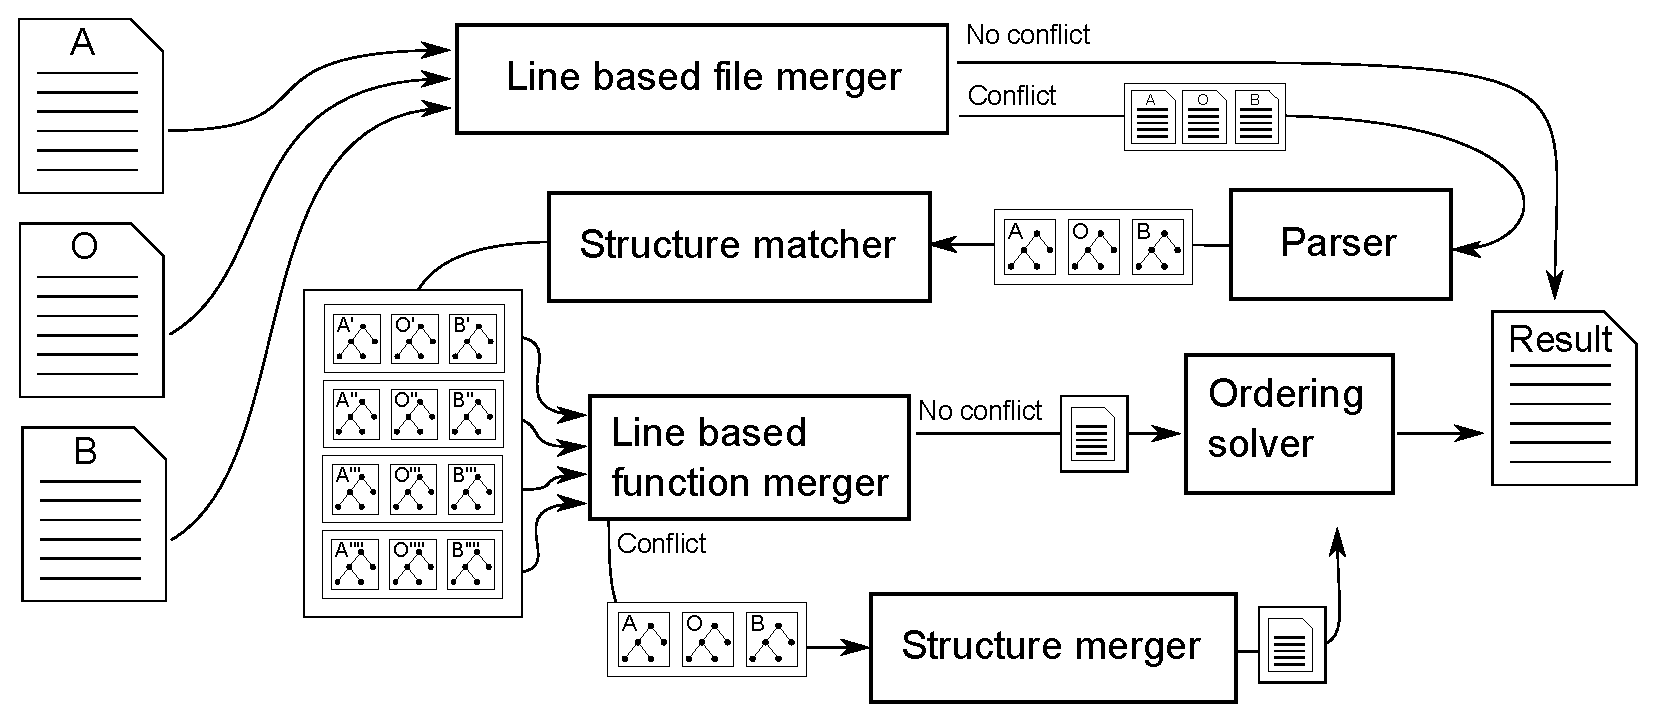
\includegraphics[scale=0.55]{drawings/eps/overallmergingprocess.eps}}
   \caption{The overall process of merging a file.}
   \label{OverallMergingProcess}
\end{figure}

\paragraph{Running time} The running time of the algorithm is the sum of the following parts:

\begin{itemize}
\item The time used by the line-based merger.
\item If it conflicts:
\begin{itemize}
\item The time spent on parsing the file and building the syntax tree.
\item The time for matching functions in a conflicting file.
\item The time it takes to line merge each function.
\item For conflicting functions, the time used on structural merging.
\item The time for reassembling in a proper order.
\end{itemize}
\end{itemize}

From a worst-case running-time perspective, this does not look good: In the worst case, we merge the entire file and hit a conflict on the last line. Then we start over, parse the files, match the functions, and try a line merge on each of these matches. Each function fail on the last line and we have to do a structure match for all of them. However, the approach is based on a couple of assumptions:

\begin{enumerate}
	\item Structure merging is much more time consuming than line-based merging.
	\item Only few files will conflict in the line-based merging, thereby launching the structural merger.
	\item When a matching is found, only few functions produce a line-based conflict, thereby launching the structural merger.
\end{enumerate}

If these assumptions hold, the overall running time is reduced considerably compared to other structured approaches, since much of our merging happens as line-merging. The first item on the list is true; both the size of the input problem and the asymptotic running time of the algorithm is larger as shown later. The second two are not as obvious to provide backing for, but best-practice guides for version control systems generally recommend that commits are small logically connected parts. Given well-encapsulated code, this means that only a few functions are changed per commit, hopefully leading to the  two assumptions being true.

\subsection{Trivial conflicts}
\label{TrivialConflict}
The goal described earlier was to minimize the amount of trivial conflicts found in the syntax tree. But what is a trivial conflict? A trivial conflict is a conflict that cannot be solved in line based tools, but where knowledge of the structure of the language allow us to make more informed choices about what is intended by the user.

\paragraph{Reordering of class-members} Class-members needs to have a definition order in concrete syntax, yet this order has no meaning for the execution in most languages. If one branch moves a method of a class, and another branch makes change to this branch, a line based tool report a conflict. An intelligent merge of this is to propagate the changes in one branches into the moved methods body.

Given a syntax tree, we know where method-definitions exists, and we can treat them as a set. This gives us a problem of matching functions together across the three branches; we need to create some heuristic that allow us to decide whether two functions are the same or not. After that we can merge the function bodies of the methods matched from the three branches.

\paragraph{Reorderings in parameter-lists and argument-lists} Parameter-lists and argument-lists are closely tied together. A reordering of the parameters in a method definition in one branch cause all argument-lists to also be reordered. If the second branch adds a parameter at the same time, this also adds an argument in all calls to this function. From a line based perspective this generates conflicts. Given a syntax tree this can be solved by matching parameters and arguments across branches and create new argument- and parameter-lists, that both contain the reorderings and the added items.

\paragraph{Merging conflicting lines} A conflict in line based tools is when two branches change the same part of the code, where there is no unchanged line inbetween those changed parts. This seems like a good heuristic for when the code for two branches might interfere, but another reason to treat this as a conflict in a line based tool, is because the tool has no idea how to merge those lines. This is however not the case for a merging algorithm based on syntax trees; we can look at sub-nodes of the trees from different branches, and merge these.

\begin{figure}

\begin{multicols*}{3}

\texttt{A}

\begin{algorithmic}
	\State $a \gets 0+2+3$
\end{algorithmic}

\columnbreak

\texttt{O}

\begin{algorithmic}
	\State $a \gets 1+2+3$
\end{algorithmic}

\columnbreak

\texttt{B}
 
\begin{algorithmic}
	\State $a \gets 1+2+4$
\end{algorithmic}

\end{multicols*}
\caption{Three statements, that conflict in a line-based merge}
\label{ConflictingLines}

\end{figure}

Given three input lines, that are vaguely similar as in figure \ref{ConflictingLines} where both branches have changed small parts of the behaviour of the line, what should we merge it into? Both branches want to change small parts of behaviour, and as such producing a conflict could easily be seen as the best choice. However re-factoring of the code like in figure \ref{RefactoredForNoConflict} makes a line based merge it without a conflict.

This show the arbitrariness of the line based merge approach; in this case it wont mean much due to it being a small integer expression, but it is easy to imagine more complicated expressions where the same refactoring makes a big difference. 

\begin{figure}
\begin{multicols*}{3}

\texttt{A}

\begin{algorithmic}
	\State $x \gets 0$
	\State $y \gets 2$
	\State $z \gets 3$
	\State $a \gets x+y+z$
\end{algorithmic}

\columnbreak

\texttt{O}

\begin{algorithmic}
	\State $x \gets 1$
	\State $y \gets 2$
	\State $z \gets 3$
	\State $a \gets x+y+z$
\end{algorithmic}

\columnbreak

\texttt{B}
 
\begin{algorithmic}
	\State $x \gets 1$
	\State $y \gets 2$
	\State $z \gets 4$
	\State $a \gets x+y+z$
\end{algorithmic}

\end{multicols*}
\caption{The lines from Figure \ref{ConflictingLines} refactored for merging without conflicts.}
\label{RefactoredForNoConflict}
\end{figure}

So what do we do? If we can match nodes in the syntax tree of the branches when they are similar, then we can do a top-down merge of nodes; we only generate a conflict when the same sub-nodes of a node has changed in both branches. This allows us to actively merge the branches in figure \ref{ConflictingLines} into $a \gets 1+2+4$ without user interaction.

\paragraph{Renaming identifiers} Local variables and class members have an identifier that is used to reference them from other places in the code. This identifier can be renamed. Renaming an identifier also has the consequence of changing the identifier all the places where this specific identifier is referenced. If a rename happens in one branch, and somebody changes or adds a line that references this identifier in another branch, the merge either give a conflict or merges perfectly, but leaves a compile error: 

\begin{itemize}
\item If somebody changes an expression around an identifier that has been renamed in another branch this generates a conflict in a line based approach. This might not produce a conflict in our approach, since we only modify parts of the sub-tree, but it might still do it.
\item If a identifier has been renamed in one branch, while somebody has added a new reference to it, in the opposite branch, this generate merge that gives an compile error.
\end{itemize}

It might be possible to detect a rename of an identifier and apply it to the trees of the other branches before doing an actual merge, and thereby avoid conflicts.

\subsection{Handling syntax trees}
\paragraph{Tree matching algorithms} Using regular tree matching algorithms on entire syntax trees takes cubic time of the number of nodes in the trees. Further, the number of nodes generated from a line of code can be high. A test on a tree generated from C\# files gave matching times of up to two minutes. This test was run on a relatively complex, but not unheard of 700-line C\# file, which gave a syntax tree with around 3800 nodes. This problem however, becomes a lot smaller if we only use it on method bodies - then it might be a viable option.

Tree matching algorithms returns a matching as a flat list of node pairs. This list makes it easy, for each node, to find the corresponding node in the other tree, and makes it possible to calculate costs easily. This can also easily be stitched together to create a three-way matching such that all nodes in the O-branch is matched with everything in the B- and A-branches.

Our goal is to construct a tree that is the merge of the branches, and here it seems there are not really a natural starting point. First of all, the merging list does not have any idea of the structure of the tree we need to construct, so the starting point needs to be an iteration over the three input-threes instead. In this iteration, however, the matching can be helpful: Whenever we encounter a change in either of the trees, we can look up the matching, and this gives us a hint about what has happened here. Resolving operations as deletions, insertions and updates is easy this way.

However, operations on trees can also be moves; nodes can be moved up or down in either of the branch trees, which makes this more complex. The matching does not tell us what happened, just that a match exists to somewhere in the other trees - this means that such an algorithm needs to search amongst parents and children to figure this out, and when this is done, produce the correct output. This might not be impossible, but the entire process becomes complex at this point. 

We abandoned the general tree matching approach, and created a matching algorithm that worked entirely on the same levels of the two input trees: Move operations are not detected up and down in the tree. This removes the above challenge. After creating such a matching, we can do a top-down recursion and create a \textit{matching tree}; a tree where each leaf is a matching between the three trees. 

The next step is to chunk these trees. Chunking is the part of the matching algorithms that divide them into stable and unstable parts, to identify updates. This definition becomes mindbogling in the matching tree generated, and we wound up abandoning the general tree-matching approach altogether.
 
\paragraph{Semantic vs. non-semantic tree-merging} A syntax-tree has a built-in semantic, that cannot be broken. Each node has some specific children with a specific type and purpose. A syntax tree can also be viewed as a tree with generic nodes with arbitrary arity. The later option is the option that allow us to run general tree-merging algorithms on the syntax trees.

Abandoning general tree merging algorithms does not mean that we have to abandon the general tree approach to merging. The advantage of using a general tree is that we can manipulate the tree more freely; for example we can insert nodes to indicate conflicts or we can create a tree iteratively instead of top-down. Further, we can create generic algorithms that work on the semantic-free trees, which then later make it easier to make the merging algorithm cross-language.

The disadvantage is that we have to create an entirely new step that takes a semantic-free-tree and turns it into a semantic tree. This step can get complicated; what should happen if a subnode has been added as a child to a node, where it does not fit semantically? This again, creates few problems.

In the end, we decided to only work on semantic trees and we decided that our algorithm should take in nodes from each branch, and return a string that corresponds to the concrete syntax created by the merge of these nodes.

\clearpage

\section{Merging and matching}
In this section we will provide several algorithm that are fundamental tools for creating our merging algorithm for syntax trees as well as the line based merge. Section \ref{UtilitiyMethods} provides functions for matching and manipulating sets and sequences generally. Section \ref{SequenceMerging} describes a general algorithm for merging sequences.  In Section \ref{EqSim} we provide functions that can decide if syntax trees are equal or similar.

The idea of two-way sequence matching, three-way sequence matching, chunking and sequence merging is based on the descriptions of \texttt{diff3} in \citet{Khanna}. We describe them more generally, since they are used for implementing our tree-merging algorithm.

\paragraph{Glossary} In this and the following sections we use some phrases, that is worth mentioning before we get started:
\begin{itemize}
\item \textbf{Base} is the original file from the version control. The file that both branches evolved from.
\item \textbf{Branch} is one of the two evolved files in the version control system.
\item \textbf{Two branches} refers to both the branches, which also often are referred to as \texttt{A} and \texttt{B}
\item \textbf{Three branches} refers to both the branches and the base file.
\item \textbf{Opposite branch} refers to the branch that was not previously mentioned. Often we will specify a condition and follow up with an action on the opposite branch; "\texttt{A} or \texttt{B} has property X and therefore we need to do Y to the the opposite branch" means "if \texttt{A} has property X, we do Y to \texttt{B}" and "if \texttt{B} has property X, we do Y to \texttt{A}".
\item For a set or a sequence, $x$, we refer to the number of items in the set, or the sequence, by $|x|$.
\end{itemize}

\subsection{Sequences and sets}
\label{UtilitiyMethods}
This section describes a series of methods that can match and manipulate sets an sequences in a way that is useful for sequence and tree merging. In some cases we motivate their existence in this section, but in other cases the motivation might first become clear in the later sections.

\subsubsection{Two-way sequence matching}
\begin{wrapfigure}{r}{0.4\textwidth}
   \centerline{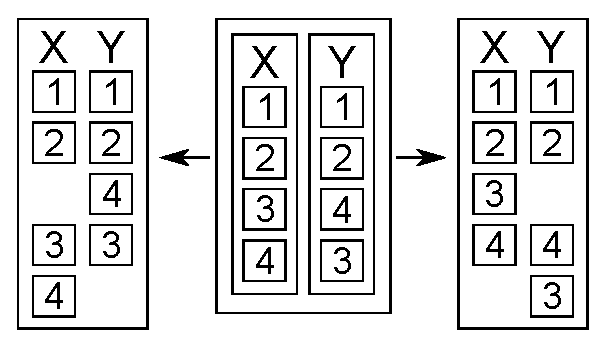
\includegraphics[scale=0.4]{drawings/eps/mincostsequencematchingambigious.eps}}
   \caption{Two input sequences that have two results from the matching algorithm.}
   \label{TwoWayMatchingAmbigiouty}
\end{wrapfigure}

Often, we want to match two sequences on their items being equal; we want to align equal elements such that we can iterate through a list that tells us whether or not an element in one sequence has a counterpart in the other.

We do this by solving the sequence alignment problem with the Needlemann-Wunsch algorithm \cite{Needleman1970443}. It allows us to minimize the penalty of alignment between two sequences, given a cost-function and a penalty for gaps in the output. In our case, we do not care about gaps in the output sequence nor do we have specific costs; all that matters is if two items are equal or not equal. The two-way sequence matching takes three parameters: Two sequences and a equality function. It runs Needlemann-Wunch with a gap-penalty at zero and the cost of equality set to -1 and the cost of inequality set to 1.

\paragraph{Result} Some inputs have several minimum-cost matchings. An example of an input that generates two different matchings can be seen in figure \ref{TwoWayMatchingAmbigiouty}.

\paragraph{Running time} The running time of Needlemann-Wunsch is often stated to be $O(n \cdot m)$, where $n$ and $m$ are the number of items in the two input sequences. This has the implicit assumption that the function that compares two items runs in $O(1)$ time. Since this function is the equality function input to our two-way sequence matching function, we do not make such an assumption; the running time is $O(n \cdot m \cdot t)$ where $t$ is the running time for the equality function.

\subsubsection{Three-way sequence matching}
\begin{figure}
   \centerline{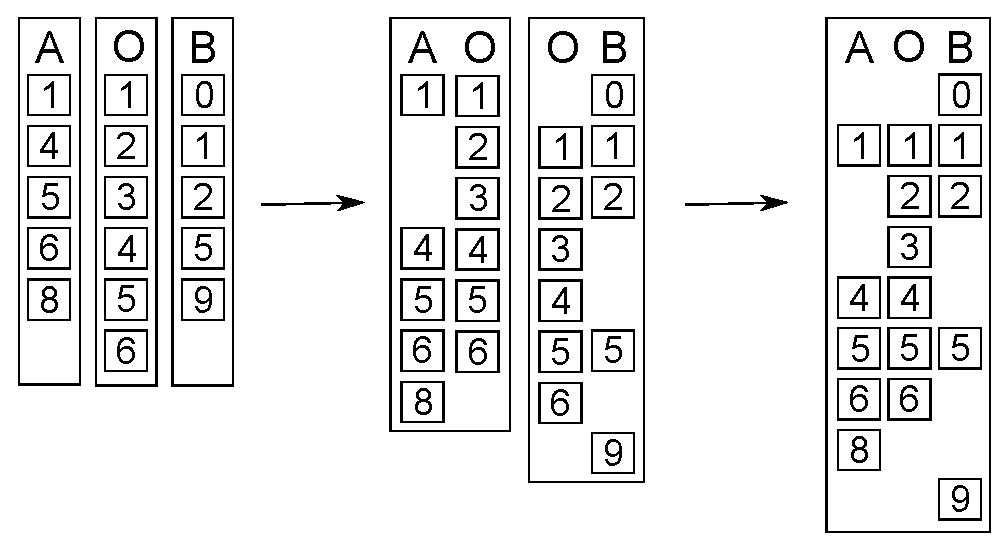
\includegraphics[scale=0.6]{drawings/eps/threewaymatching.eps}}
   \caption{A run of the Three-way matching-algorithm}
   \label{ThreewayMatching}
\end{figure}

\begin{algorithm}
\begin{algorithmic}
\Function{ThreeWayMatching}{$A$, $O$, $B$, $equality$}
	\State $m_a\gets$ TwoWayAllign($A, O, equality$)
	\State $m_b\gets$ TwoWayAllign($B, O, equality$)
	
	\State $a \gets 0$
	\State $b \gets 0$
	\State $r \gets [\,]$
	
	\While{$a+b < |m_a| + |m_b|$}
		\If{$a \geq |m_a|$ or $b \geq |m_b|$}
			\State add item from opposite matching to $r$
			\State increase opposite counter
		\ElsIf{$m_a[a].o$ is null or $m_b[b].o$ is null}
			\State add the matching whose $o$-item is null to $r$
			\State increase that matchings counter
		\Else
			\State add $m_a[a]$ and $m_b[b]$ to $rv$
			\State increase $a$ and $b$
		\EndIf
	\EndWhile
	\State \Return $r$
	
\EndFunction
\end{algorithmic}
\caption{Three-way matching algorithm}
  \label{ThreeWayMatchingAlgorithm}
\end{algorithm}

Given three input sequences A, O and B, we want to output a single sequence of matchings between them. A match is a data-structure, that contains three elements A, O and B, illustrated as a row in the result of Figure \ref{ThreewayMatching}. An empty result in any of the three columns on each row means that there is no matching from this specific input sequence.

As can be seen in Algorithm \ref{ThreeWayMatchingAlgorithm}, we perform two two-way sequence-matchings on the sequence-pairs $(A, O)$ and $(O, B)$, this results in two sequences of matchings.  We iterate over these matchings in parallel; starting at the first item of both and continuing to the next item of a specific matching in the following circumstances:

\begin{itemize}
	\item If either of the matchings are at the end of the sequence, add the opposite item to the result and iterate further in that matching sequence.
	\item If either of the matchings has matched a \textit{null} from the $O$-sequence, add this item to the result and iterate further in that matching sequence.
	\item Otherwise the item from the $O$-sequence must be the same in both matchings, and we can add both items to the result and iterate to the next item in both matching sequences.
\end{itemize}

Each column in a matching keeps the order of the input sequences, and the intuition behind the $while$-loop in the algorithm is that the $O$-items in the two matching always show up in order.

\paragraph{Running time} The running time for the two-way alignment functions are $O(|A||O|t)$ and $O(|B||O|t)$, where $t$ is running time for $equality$. These function results in two lists, maximally of the size $|A|+|O|$ and $|B|+|O|$ --- in the case where no matching exists. The \textbf{while}-loop iterate at most $|A|+|O|+|B|$ times, and all operations inside it are constant time. This gives an upper bound running-time of:

\begin{equation}
	O(|A||O| t + |B||O| t ) \nonumber
\end{equation}  


\subsubsection{Chunking}

\begin{algorithm}
\begin{algorithmic}
\Function{Chunking}{$matching$}
	\State $cs \gets matching.ChunkBy($no items in a matching are null$)$
	\State $r \gets [\,]$
	\ForAll{$c$ in $cs$}
		\State $chunk \gets $ init new chunk
		\ForAll{$m$ in $c.matches$}
			\If{$m.A \neq $ null}
				\State $chunk.A.Add(m.A)$
			\EndIf
			\If{$m.O \neq $ null}
				\State $chunk.O.Add(m.O)$
			\EndIf
			\If{$m.B \neq $ null}
				\State $chunk.B.Add(m.B)$
			\EndIf
		\EndFor
		\State $r$.add($chunk$)
	\EndFor
	\State \Return $r$
\EndFunction
\end{algorithmic}
\caption{Chunking algorithm}
  \label{CunkingAlgorithm}
\end{algorithm}

\begin{wrapfigure}{r}{0.5\textwidth}
   \centerline{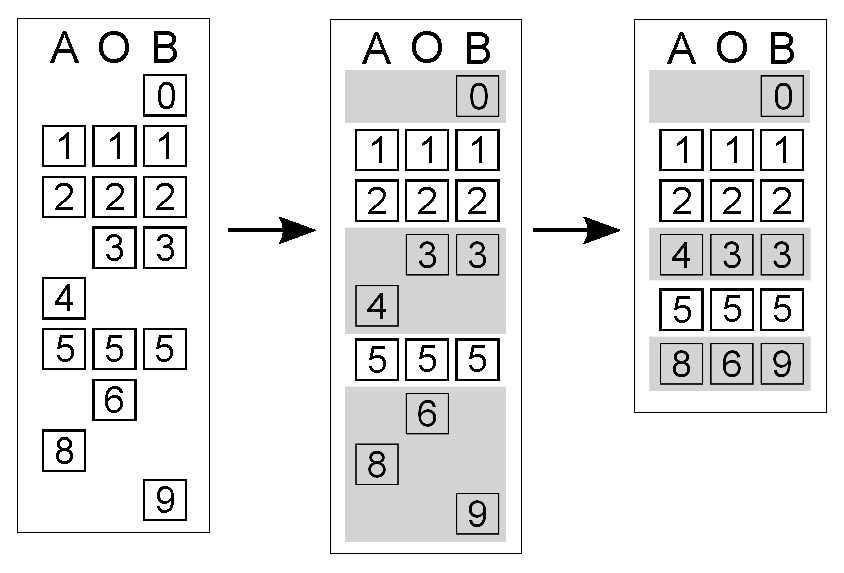
\includegraphics[scale=0.4]{drawings/eps/threewaymatching-chunking.eps}}
   \caption{Chunking a matching. Grey areas are unstable chunks and white areas are stable.}
   \label{Chunking}
\end{wrapfigure}

Given a three-way sequence matching, a single match can be defined as \textit{stable} or \textit{unstable}; if a matching has been found in all input sequences $A$, $O$ and $B$ it is stable. Otherwise it is unstable. This notion is quite useful for performing a merge; it is reasonable to assume that a stable match, does not need to be merged.


Another view could be that an unstable match should be viewed as either a deletion or an insertion. This however leaves us in a situation where all matchings can easily be resolved into a merge; something is inherently wrong with that approach. The problem is that the matching sequence cannot represent the actual sentiment of the changes it is seeing: A deletion followed by an insertion might be an update of a single line. If both branches have done an update of the same line, then a conflict should be produced. Because of this we need to introduce \textit{chunking}.

A chunk is three lists, one for A, one for O and one for B. A chunk can be stable or unstable. Given a sequence matching, we generate a list of chunks by iterating over every single matching. If the first element is stable, then we generate a stable chunk, and add its three items to the appropriate list. We continue adding all elements until we hit an unstable match. When we hit an unstable match, we generate an unstable chunk and add all non-empty elements from the match to the appropriate list.

The pseudocode for this algorithm is in Algorithm \ref{CunkingAlgorithm}. \footnote{The ChunkBy method used in the algorithm can be found at \url{http://msdn.microsoft.com/en-us/library/cc138361.aspx}}

\paragraph{Result} The result is a sequence of alternating stable and unstable chunks, containing all the items that was provided in the input matching. Notice that unstable chunks not necessarily are conflicts; in the result in Figure \ref{Chunking} the top item is an insertion of the $0$-item. The second chunk is an update where $3$ is turned into $4$. Only the last chunk is a conflict, since both A and B has changed the representation. 

\paragraph{Running time} The ChunkBy-method only performs constant time operations on each element in the input sequence, and we can conclude that it is running in $O(n)$ time, where $n$ is the number of items in the input matching. The number of chunks is unknown without looking at the input, however the total number of matches within all the chunks is $n$. Therefore the upper bound running time is $O(n)$ for the entire chunking-process.

\subsubsection{Priority-chunking}
\label{PriorityDiff}

\begin{algorithm}
\begin{algorithmic}
\Function{PriorityChunk}{$A$, $O$, $B$, $equal$, $similar$}
	\State $m \gets \Call{ThreeWayMatching}{A, O, B, equal}$
	\State $c' \gets \Call{Chunking}{m}$
	\State $r \gets [\,]$
	\ForAll{$c$ in $c'$}
		\If{$c$ is stable}
			\State add $c$ to $r$ as equality-stable
		\Else
			\State $m' \gets \Call{ThreeWayMatching}{c.A, c.O, c.B, similar} $
            \State $cs' \gets \Call{Chunking}{m'}$
			\ForAll{$c'$ in $cs'$}
				\If{$c'$ is stable}
					\State add $c'$ to $r$ as similar-stable
				\Else
					\State add $c'$ to $r$ as unstable
				\EndIf
			\EndFor
		\EndIf
	\EndFor
	\State \Return $r$
\EndFunction
\end{algorithmic}
	\caption{Priority-chunking algorithm}
	\label{PriorityChunk}
\end{algorithm}

Our three-way matching function operates on equality. Yet in some cases we want to use heuristics functions that looks for similar items instead of absolute equality. To use such a heuristic function in the matching functions earlier defined, it has to answer either "similiar" or "not similar", and cannot distinguish between equality and similarity. However, sometimes we want to make sure that completely equal items are matched before similarity is used.

The solution to this problem is priority-chunking as shown in Algorithm \ref{PriorityChunk}. It starts by doing a matching on the three input sequences using a strict equality function. It then iterates through all chunks and for unstable chunks it does another matching using the similarity-function, and generates three types of chunks:

\begin{itemize}
   \item Equality-stable items; items that we matched as stable by the \textit{equal}-function.
   \item Similarity-stable items; items that we matched as stable by the \textit{similar}-function.
   \item Unstable items; items that was not matched as stable.
\end{itemize}

\paragraph{Running time} A crude upper bound analysis of the running time for algorithm can be done like this: The first ThreeWayMatching function is  $O(|A||O|t + |B||O|t)$ and it returns maximally $A+O+B$ items, which are then passed to the chunking function, which run in $O(n)$ time. This gives a worst case running time like below, for the first two statements in the algorithm.

\begin{equation}
O(|A||O|t + |B||O|t + |A|+|O|+|B|) \nonumber
\end{equation}

The for-loop around $chunks$ runs $|A|+|O|+|B|$ times in worst case. In each iteration the worst case running time is the same as above. This gives this worst case running time for the loop:

\begin{equation}
O((|A| + |O| + |B|) (|A||O|t' + |B||O|t' + |A|+|O|+|B|)) \nonumber
\end{equation}

However, this describes the situation where every single chunk contains the entire input matching. This is obviously not true. It can be seen that:

\begin{enumerate}
\item If there are $|A|+|O|+|B|$ chunks, then the running time of ThreeWayMatching is $O(1)$
\item If there is 1 chunk, then the running time of the inner ThreeWayMatching is the same as for the outer ThreeWayMatching.
\end{enumerate}

A more accurate way of describing the running time of the \textbf{for}-loop of Algorithm \ref{PriorityChunk} is the sum over each chunk, and their individual sequences from each input branch $c_a$, $c_o$ and $c_b$:

\begin{equation}
\sum_{c \in C} O(|c_a||c_o|t' + |c_b||c_o|t' + |c_a|+|c_o|+|c_b|) \nonumber
\end{equation}

We know that each chunk contains only items from the input sequences, and we know there is no overlap between chunks. Therefore, we know that:

\begin{equation}
\sum_{c \in C} |c_a| = |A| \nonumber
, \sum_{c \in C} |c_o| = |O| \nonumber
, \sum_{c \in C} |c_b| = |B| \nonumber
\end{equation}

This means that we can simplify the above sum by moving out the sums:

\begin{equation}
O(|A| + |O| + |B| + \sum_{c \in C} |c_a||c_o|t' + |c_b||c_o|t)' \nonumber
\end{equation}

We also know that:

\begin{equation}
\sum_{c \in C} |c_a||c_o| \leq |A||O| , 
\sum_{c \in C} |c_b||c_o| \leq |B||O| \nonumber
\end{equation}

And thereby we can upper bound the above as:

\begin{equation}
O(|A| + |O| + |B| + (|A| |O| + |O| |B|) t') \nonumber
\end{equation}

This leaves us with the overall running time of:

\begin{equation}
O((|A| + |B|)|O|t + |A|+|O|+|B| + (|A| |O| + |O| |B|) t')) \nonumber
\end{equation}

Where $t$ is the running time of $equal$ and $t'$ is the running time of $similar$. This can be simplified into:

\begin{equation}
O(|O| (|A| + |B|)(t + t')) \nonumber
\end{equation}

\subsubsection{Two-way set matching with costs}
Finding a minimum cost matching of the bipartite sets \texttt{x} and \texttt{y} can be solved in cubic time using a maximum flow algorithm as described by \citet{bipartitecost}. A prerequisite of this algorithm is however that the two sets are equal in size. Further, it assumes that the input can generate a perfect matching in the internal graph. We want to modify the bipartite graph algorithm such that it can consume differently sized sets, and generate the best minimum cost matching, even though there is no perfect matching.

The \citet{bipartitecost} algorithm starts by generating a weighted undirected graph, $G$. In this graph each item of the input sets is a node in the graph, and for each pair of nodes an edge is generated with the cost between them as the weight. The algorithm defines a set of prices $p$ for each nodes. For $x$-nodes the initial prices are initially 0 and for $y$-nodes the initial prices is equal to the minimum weight of the incoming edges. It then creates a residual graph $G_M$ given a matching. The residual graph contains all the nodes of the original graph $G$, and further a source node $s$, and a sink node $t$. The source node has zero-cost edges to all $x$-nodes not in the matching and each $y$-node has a zero-cost edge towards the sink not in the matching. For each edge in the original graph, we add an edge in the residual graph - if this specific edge exists in the matching we add it as an edge from $y$ to $x$, otherwise from $x$ to $y$. The price weight of these edges is the $price(xnode)+originalgraphweight-price(ynode)$. For each iteration of the algorithm it updates the prices such that the price in the next iteration is the current price and the cost to get from source to this node in the current residual graph.

The pseudocode for the algorithm can be found in Algorithm \ref{OriginalCostMatching}.


\begin{algorithm}
\begin{algorithmic}
\Function{BipartiteSetMatching}{$X$, $Y$}
	\State Generate $G$ from $X$ and $Y$ given a cost function
	\State Start with $M$ equal to the empty set
	\State Define $p(x)$ for $x \in X$, and  $p(y) = \underset{e \; into \; y}{\operatorname{min}} c_e$ for $y \in Y$
	\While{$M$ is not a perfect matching}
    	\State Find a minimum-cost $s-t$ path $P$ in $G_M$ with prices $p$
    	\State Augment along $P$ to produce a new matching $M'$
    	\State Find a set of compatible prices with respect to $M'$
    \EndWhile
	\State \Return $M$
\EndFunction
\end{algorithmic}
	\caption{Bipartite set matching algorithm}
	\label{OriginalCostMatching}
\end{algorithm}

We want to modify this algorithm to have the following properties:

\begin{itemize}
\item It should work for x and y sets of different size. 
\item It should work even though a perfect matching cannot be found in the residual graph.
\item For any element not matched it should return a matching $(x, \epsilon)$ or $(\epsilon, y)$
\end{itemize}

If the sets are not equal in size, we add nodes, auxiliary nodes, in the smallest of the two sets until the two sets are equal in size.\footnote{This concept is derived from a project I did in autumn 2012 with Torben Andersen} For each auxiliary node we add an edge to each node in the opposing set with a cost larger than the largest cost between any other pair of nodes. In the final matching, the matchings that contain auxiliary nodes should be considered as not matched; since they have been matched with the highest possible weight for their edges - the rest of the matchings are definitely the minimum cost matching.

The second challenge is due to the fact that the end-condition in the loop requires a perfect matching. However if any node in any of the two sets does not have a cost defined for a single node in the opposite set, then a perfect matching is not possible. An example of such a situation could be $X={1, 2}$ and $Y={1, 3}$ with a cost function only defined for elements that are numerically equal. This is demonstrated below. \\

\begingroup
    \fontsize{7pt}{10pt}\selectfont
\begin{tabular}{ p{5.5cm} | p{5.5cm} }
   \centerline{\includegraphics[scale=0.3]{drawings/eps/TwoWayCostMatchingNotPerfect/1it0.eps}} &
    \centerline{\includegraphics[scale=0.3]{drawings/eps/TwoWayCostMatchingNotPerfect/1it1.eps}} \\
   Initial graph for the sets and cost function. &
    The first residual graph. \\ \\ \hline \\

    \centerline{\includegraphics[scale=0.3]{drawings/eps/TwoWayCostMatchingNotPerfect/1it2.eps}} &
    \centerline{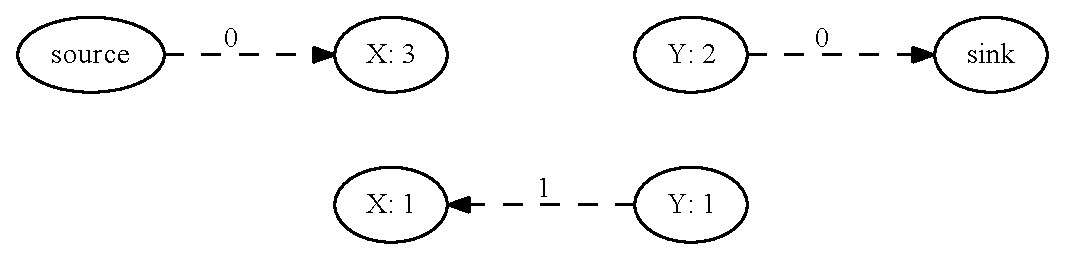
\includegraphics[scale=0.3]{drawings/eps/TwoWayCostMatchingNotPerfect/1it3.eps}} \\
   Running Dijkstra finds a matching. &
   In the second residual graph, all possible matchings have been found, but the matching is still not a perfect matching. \\ 
\end{tabular}

\endgroup

When our algorithm reaches the second iteration, the matching is still not perfect for the entire graph. The problem is that one or more edges have no edges in the initial graph. The solution is to only generate nodes if a cost defined for any other node. The result for nodes without a cost generated, will be the node itself and a empty match in the opposite set. This is obviously a correct assumption; since they have no costs associated to the other set, they are of course impossible to match.

Looking at the same example, now that the node $(X: 1)$ has a cost to the node $(Y: 2)$. For this graph a perfect matching is not possible either. The problem is solved by deleting nodes with no cost, and afterwards generating auxiliary nodes; as seen in the right figure below. \\

\begingroup
    \fontsize{7pt}{10pt}\selectfont
\begin{tabular}{ p{5.5cm} | p{5.5cm} }
   \centerline{\includegraphics[scale=0.3]{drawings/eps/TwoWayCostMatchingNotPerfect/NoFakeNode.eps}} &
    \centerline{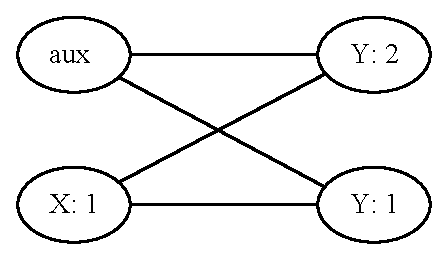
\includegraphics[scale=0.3]{drawings/eps/TwoWayCostMatchingNotPerfect/FakeNode.eps}} \\
   A graph where all nodes have a cost, but where no perfect match is possible. &
    The same graph, with auxiliary nodes added to make a perfect match possible. \\ 
\end{tabular}

\endgroup

We now have three sets, that together be the final matching:
\begin{itemize}
   \item The matchings that have an original input item in both ends.
   \item The matchings that have an auxiliary node in either end.
   \item The set of nodes that were never added to the graph.
\end{itemize}

We union the above sets. When doing so, we generate matching where one of the two items of the matching is empty, for the last two bullets in the above list. The algorithm can be seen in Figure \ref{TwoWayCostMatching}.

\paragraph{Running time} The running time for the original algorithm is expressed in terms of the input size of both sets $n$ as $O(n^2 \log n)$. We have artificially expanded the smaller of the two sets. Therefore $n$ is $\max(|X|, |Y|)$ in our case, and the running time is:

\begin{equation}
O(\max(|X|, |Y|)^2 \log (\max(|X|, |Y|)) \nonumber
\end{equation}

\begin{algorithm}
\begin{algorithmic}
\Function{TwoWayCostMatching}{$X$, $Y$}
	\State Generate $G$ from $X$ and $Y$ given a cost function.
	\State ~~~~ Store items of $X$ and $Y$ that has no cost.
	\State ~~~~~~ Do not add them to $G$.
	\State ~~~~ Inserting auxiliary nodes if the $|X| \neq |Y|$


	\State Start with $M$ equal to the empty set
	\State Define $p(x)$ for $x \in X$, and  $p(y) = \underset{e \; into \; y}{\operatorname{min}} c_e$ for $y \in Y$
	\While{$M$ is not a perfect matching}
    	\State Find a minimum-cost $s-t$ path $P$ in $G_M$ with prices $p$
    	\State Augment along $P$ to produce a new matching $M'$
    	\State Find a set of compatible prices with respect to $M'$
    \EndWhile
    
	\State $r \gets $  $(x, \epsilon)$ or $(\epsilon, y)$ for each matching containing an auxiliary node $\cup$
    \State ~~~~~ $(x, \epsilon)$ or $(\epsilon, y)$ for each item not added to $G$ $\cup$
    \State ~~~~~ all matchings not containing auxilary nodes 
    \State \Return $r$
\EndFunction
\end{algorithmic}
\caption{Two-way set matching algorithm}
\label{TwoWayCostMatching}
\end{algorithm}


\subsubsection{Three-way set matching with costs}

\begin{algorithm}
\begin{algorithmic}
\Function{ThreeWayCostMatching}{A, O, B, $\texttt{cost}$}
	\State $m_a\gets \Call{TwoWayCostMatching}{$A, O, $\texttt{cost}}$
	\State $m_b\gets \Call{TwoWayCostMatching}{$B, O, $\texttt{cost}}$
	
	\State Sort $m_a$ after the index of $O$-items
	\State Sort $m_b$ after the index of $O$-items

	\State $a \gets 0$
	\State $b \gets 0$
	
	\State $r \gets []$
	
	\While{$a+b < |m_a| + |m_b|$}
		\If{$a \geq |m_a|$ or $b \geq |m_b|$}
			\State add item from opposite matching to $r$
			\State increase opposite counter by $1$
		\ElsIf{$m_a[a].o$ is null and $m_b[b].o$ is null}
			\State add the $m_a[a]$ to $r$
			\State add the $m_b[b]$ to $r$
			\State increase $a$ and $b$ by $1$
		\Else
			\State add $(m_a[a], m_b[b])$ to $r$
			\State increase $a$ and $b$ by $1$
		\EndIf
	\EndWhile
	\State \Return $r$
\EndFunction
\end{algorithmic}
\caption{Three-way set matching algorithm}
  \label{ThreeWayCostMatchingAlgorithm}
\end{algorithm}

When we are given an original set $O$ and two branched sets $A$ and $B$, three way cost-matching allows us to decided what items of each set belong together if we define a decent cost-function. We sort the output matching after the index of their input $O$-items, to align all items that have been matched in all three sets. We then iterate through the sequences, and add them as unmatched in their opposite branch, or add the matching from both branches to the result list. Algorithm \ref{ThreeWayCostMatchingAlgorithm} shows this.

\paragraph{Running time} The two two-way cost matching algorithms runs in $O(m_{a}^2 \log m_{a})$ and $O(m_{b}^2 \log m_{b})$ time, where $m_{a}$ is $\max(|A|, |O|)$ and $m_{b}$ is $\max(|B|, |O|)$. They return sequences of the maximal sizes $A+O$ and $O+B$. Ordering each of the matchings takes $O(n \log n)$ time; which overall gives $O((A+O) \log (A+O) + (B+O) \log (B+O))$. Afterwards we iterate through $A+O+B$ items, and for each of them do constant time operations.

This gives us the overall time of:
\begin{equation}
O(m_{a}^2 \log m_{a} + m_{b}^2 \log m_{b} + (A+O) \log (A+O) + (B+O) \log (B+O) + A + O + B) \nonumber
\end{equation}

If we define $n$ as $\max(|A|, |O|, |B|)$, which is clearly an upper bound, the expression can be simplified to:

\begin{equation}
O(n^2 \log n + n \log (n) + n) \nonumber
\end{equation}

And further to:

\begin{equation}
O(n^2 \log n) \nonumber
\end{equation}

\subsubsection{Reordering}
\label{ThreeWayReorderingAlgorithmSec}

\begin{algorithm}
\begin{algorithmic}
\Function{Reordering}{$A$, $O$, $B$}
   \State $ms \gets \Call{ThreeWayMatcing}{A, O, B, $ item equalilty $}$
   \State $r \gets [\,]$
   
   \ForAll{$m$ in $ms$}
      \If{$m$ is insertion}
         \State add relevant item (A or B) to $r$.
      \EndIf
      \If{$m$ is move and exists in opposite branch}
         \State add relevant item (A or B) to $r$.
      \EndIf
      \If{$m$ is unchanged}
         \State add item O to $resultList$
      \EndIf
      
	\EndFor
	\State $c \gets$ find indexes of duplicate items in $r$
	\State \Return $(r, c)$
\EndFunction
\end{algorithmic}
\caption{Three-way reordering algorithm}
  \label{ThreeWayReorderingAlgorithm}
\end{algorithm}


Several times in this thesis, we match sets together and afterwards want to produce a sequence for our output. While we are looking at the sets, we have no order, and when we later want to produce the sequence we will have to generate this order. Here we provide a function to resolve the problem where reordering of items in a sequence have happened in different branches. We define a general three-way sequence-reordering-function. Given an original sequence and two reordered sequences, the result is a single sequence where all elements are outputted in a order that can reasonably be described as a merge of the orders in the three input sequences.

Reorderings can conflict. One example could be that the sequence \texttt{(a, b, x, c, d)} has turned into \texttt{(x, a, b, c, d)} in one branch and \texttt{(a, b, c, d, x)}. These three sequences can easily be intepreted as \texttt{x} being been moved different places in the two branches, and a conflict should be produced.

If one branch moves an item and the other branch deletes it, we interpret this as a deletion. This might not be completely intuitive. Our reason this, is in the knowledge of how the reordering function will be used; to reorder class members or function parameters. If one branch removes a parameter, this has also the consequence that the function body will no longer refer to this parameter. If another branch simply reorders it; they have expressed no reason to keep it. The same idea holds for function definitions in class members; their order is semantically meaningless, and if it is removed from one branch then all references for this class member are also removed in this branch.

To do a three-way reordering, the obvious entry point is to identify which items have been moved, and then apply all these moves to the output sequence. This however leads to quite a few non-trivial definitions. How do we describe a move? It might be described by an item of the input sequences, but how do we define the place that it should be moved to? Several options are available: Insert after or before a specific item, insert between items or insert at a particular index, and many more. Each of these options, however present further complications. If we choose to insert something after an item, in the output sequence, then do we do that before or after we move that item?

Further, such a move operation is not our input, and it is not clear how to calculate one from our input. Our input is three sequences with a specific order, and given those, many different move operations could be generated. The difference between two sequences \texttt{a, b, c, d} and \texttt{a, b, d, c} can be interpreted as \texttt{c} being moved to after \texttt{d}, as \texttt{d} being placed before \texttt{c}, as \texttt{c} and \texttt{d} swapping places, and many other options. Also, figuring out the correct representation of a move in an algorithmic way can only be an uninformed guess - the users reasoning for doing a reordering is probably grounded in context that the algorithm is unaware of.

We interpret reorderings differently. Given the input sequences we do three-way matching. Such a matching produces the actual ordering. A matching contain some stable elements and some unstable elements. The stable elements are elements where a match exists in both A, O and B. we assume these elements to be items that have not moved in the sequence. If something is not stable, it is either a \textit{move}, an \textit{insertion} or a \textit{deletion} as seen in Table \ref{ReorderingTable}.

\begin{table}

\centering
\begin{tabular}{ | l | l | l || r |}
  \hline                        
   \textbf{A} & \textbf{O} & \textbf{B} & \textbf{Action by user} \\
  \hline                        
  Empty & Value & Value & \textit{Moved from} or \textit{deleted} in A \\
  Value & Value & Empty & \textit{Moved from} or \textit{deleted} in B \\
  Value & Empty & Empty & \textit{Inserted} or \textit{moved to} in A \\
  Empty & Empty & Value & \textit{Inserted} or \textit{moved to} in B \\
  Value & Value & Value & Unchanged \\
  \hline  
\end{tabular}
  \caption{How to interpret matchings in the reordering algorithm}
\label{ReorderingTable}
\end{table}

We iterate through each matching, and treat them as such. Distinguishing between a \textit{deletion} or a \textit{move from} is not important - neither should be added to the output. However, distinguishing between \textit{insertion} and \textit{move to} is important. Insertions should always be inserted in the output, however moves should only be inserted to the output if they have not been deleted in the opposite branch. 

A conflicting move is a move where two \textit{move to} operations exists on each list. Detecting these is a matter of looking into duplicate records in the resulting list. These are returned along with the result, and the callers of the reordering methods have the responsibility of presenting these to the user.

\begin{figure}
   \centerline{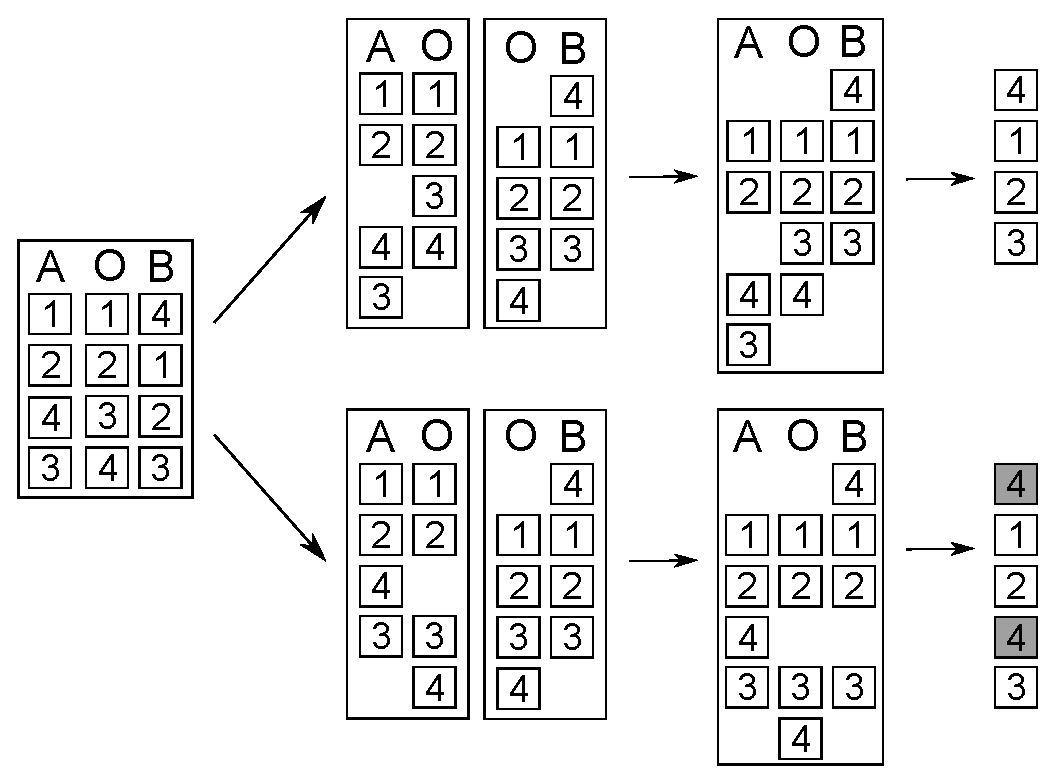
\includegraphics[scale=0.55]{drawings/eps/reordering.eps}}
   \caption{Two possible outcomes of the reordering algorithm. Gray items in the result are conflicts.}
   \label{Reordering}
\end{figure}

The process of reordering can be seen in Figure \ref{Reordering}. This figure also shows that the ambiguity in our two-way-matching algorithm can lead to different potential outcomes of the reordering algorithm; if the \texttt{AO}-matching chooses to match the 4, implying that 4 has only moved in the \texttt{OB}-match, then we produce a conflict-free output. If the \texttt{AO}-matching chooses 3 as the match, we get a conflict where 4 is being inserted both places. The safe bet is to modify the algorithm such that a conflict is always produced, by modifying the two-way-matching to return all possible matchings, and let the three-way-matching algorithm choose a pair that share most matchings.

\paragraph{Running time} ThreeWayMatching runs in $O(|A||O| t + |B||O| t)$ time, where $t$ in this case is constant time for checking referential equality. In worst case it returns $|A|+|O|+|B|$ items. The loop in the algorithm contains constant time operations which means the overall running time is $O(|A|+|O|+|B|)$ for the loop. Conflict detection can be done by keeping a hash set on the side of the results already added which gives us constant time lookup for each item, leaving us with $O(|A|+|O|+|B|)$ time.

The reordering algorithm has the following upper bound running time:

\begin{equation}
O(|A||O| + |B||O|) \nonumber
\end{equation}


\subsection{Sequence-merging}
\label{SequenceMerging}

\begin{algorithm}
\begin{algorithmic}
\Function{MergeSequence}{$\texttt{A}$, $\texttt{O}$, $\texttt{B}$, \texttt{equality}, \texttt{conflicthandler}}
   \State $\texttt{match} \gets \Call{ThreeWayMatch}{\texttt{A}, \texttt{O}, \texttt{B}, \texttt{equality}}$
   \State $\texttt{chunks} \gets \Call{Chunking}{\texttt{match}}$
   \State $\texttt{merged} \gets [\,]$
   \ForAll{\texttt{chunk} in \texttt{chunks}}
        \If {\texttt{chunk} is stable}
            \State add line of chunk.O to merged
            \State continue to next iteration
        \EndIf
        \If {\texttt{chunk} is added in \texttt{A} or \texttt{B }}
            \State add lines of \texttt{chunk} to \texttt{merged}
        \Else
            \If{\texttt{O} is equal with one branch, but not the other}
               \State add lines of changed branch to \texttt{merged}
            \ElsIf{the two branches are equal}
               	\State add either of them to merged
			\Else
				\State \Call{conflicthandler}{\texttt{merged}, \texttt{chunk}}
				\If{conflict-handler indicates termination}
					\State break
                \EndIf
			\EndIf
   		\EndIf
    \EndFor
	\State \Return \texttt{merged}
\EndFunction

\end{algorithmic}
\caption{Sequence merging algorithm}
  \label{Genericmergingalgorithm}
\end{algorithm}

The sequence based merging algorithm from Algorithm \ref{Genericmergingalgorithm} is based on the description found of the original \texttt{diff3} algorithm in \citet{Khanna}. Conflict-handling is delegated to an input function, to allow different handling in different situations. We pass the list of current merged text, and the currently unmerged chunk. The merged list can be arbitrarily modified inside the conflict handler. We also allow the conflict handler to break out of the entire loop. This supports two essential use-cases:

\begin{itemize}
   \item Output the three items of the chunk, indicating that these are conflicting.
   \item Clear the merged list inside the conflicthandler, and start over with a different merging algorithm.
\end{itemize}

\paragraph{Running time} Three-way matching and chunking gives us an upper bound running time of $O(|A||O| t + |B||O| t + |A|+|O|+|B|)$, given that $t$ is the running time of $equality$. The loop runs $|A|+|O|+|B|$ times. All operations inside the loop are constant time, except for the conflict-handler which has an unknown running time. The above two use cases can also be divided into two scenarios for the conflict-handler:

\begin{itemize}
	\item When the conflict-handler output the chunks as conflicting, it runs only constant time operations on the chunks, for any chunk. The running time is:\\
		\begin{equation}
			O(|A||O| t + |B||O| t) \nonumber
		\end{equation}

	
	\item When the conflict-handler flushes the output and starts a new merging algorithm it also break the loop, meaning conflicthandler is only invoked once. Given that $t'$ is the time it takes to run the conflicthandler, the running time is:\\
		\begin{equation}
			O(|A||O| t + |B||O| t + t') \nonumber
		\end{equation}

\end{itemize}


\subsection{Equality and similarity}
\label{EqSim}
In this section we define equality and similarity on syntax trees. Equality and similarity are important for matching algorithms; these are the function that will define whether or not a matching will happen or not.

Equality is important to allow for exact comparison between trees, and similarity is important because it allows us to match trees that are not completely equal but are close enough to allow a tree-based merge.

\subsubsection{Equality}
The equality function defines whether or not two nodes taken from syntax-trees in different branches are equal to each other.

If we view syntax trees as n-ary trees with no semantic meaning, this becomes easy. Every node has a label and $n$ children. Given two nodes $x$ and $y$ we need to check if the label is equal, and we need to iterate through each pair of children on the same index. Whenever we encounter something not equal, return false. Otherwise return true.

\paragraph{Running time} The worst case running time for the equality algorithm is the case where two trees are completely equal; in this case we will have to visit every single node to verify the equality. The upper bound for the running time becomes $O(n)$ where $n$ is the amount of nodes in the tree.

\subsubsection{Similarity}
\label{FunctionSimilarity}

\begin{algorithm}
  \caption{Node similarity algorithm}
  \label{SimilarityAlgorithm}
\begin{algorithmic}
\Function{NodeSimilarity}{\texttt{x}, \texttt{y}}
	\If{(\texttt{x} or \texttt{y} is \texttt{null}) or (\texttt{x} or \texttt{y} are different types)}
		\State \Return 0
	\ElsIf{\texttt{x} and \texttt{y} are fixed structural nodes}
		\State \Return average of \Call{NodeSimilarity}{} of children
	\ElsIf{\texttt{x} and \texttt{y} are tokens}
		\State \Return $ \text{x} = \text{y}$ ? 1 : 0
	\ElsIf{\texttt{x} and \texttt{y} are argumentlists}
		\State \texttt{m} $\gets$ \Call{TwoWayCostMatch}{\texttt{x}, \texttt{y}, expression equal}
		\State \texttt{c} $\gets$ \Call{Map}{} (\texttt{m}, (\texttt{x}, \texttt{y}) $\rightarrow$ \texttt{x} or \texttt{y} is null ? 0 : 1)
		\State \Return \Call{Average}{\texttt{Cost}}
	\ElsIf{\texttt{x} and \texttt{y} are blocks}
		\State \texttt{m'} $\gets$ \Call{TwoWayAllign}{x, y, equal}
		\State \texttt{s} $\gets$ 0, \texttt{t} $\gets$ 0
		\ForAll{\texttt{m} in \texttt{m'}}
			\If{\texttt{m}$_x$ is null or \texttt{m}$_y$ is null}
				\State \texttt{s} += 1
			\Else
				\State \texttt{s} += 2
				\State \texttt{t} += 2
			\EndIf
		\EndFor
		\State \Return $ \texttt{s} / \texttt{t} $;
	\EndIf
\EndFunction
\end{algorithmic}
\end{algorithm}


Similarity should return whether two nodes are similar or not. We divide it into two functions:  One that decides a similarity percentage between two nodes. Around this function we define a function that thresholds this percentage.

\paragraph{Initial assumptions} Is the expression $x=1+2+3$ similar to $f(1+2+3)$? They have atleast 5 nodes in common; three integers and two add operators - this, out of 7 nodes in total. From that perspective they seem quite similar. For several reasons, we decide that only syntax-nodes of equal type should be considered similar:

\begin{enumerate}
\item As noted by \citet{Hashimoto}, showing a fine grained difference, might be more confusing than showing the two statements as an insertion and deletion.
\item The running time of creating the matchings become considerably larger if every single sub-tree has to be compared to all other sub-trees  for similarity.
\item The complexity of the merge algorithm is considerably less, if we can assume that children of any of the input nodes are always the same. This is also the case for the similarity function itself.
\item If we want to allow for merging of the above cases, this can still be done, in the same way that we allow of uneven tree merging when no other ways of resolving an update is possible: It generates an unstable chunk. Given this chunk we can match the sub-trees much quicker because we have a much more narrow field for the matching.
\end{enumerate}

Given that two nodes are only equal if they are of the same node-type, most of the similarity is quite straightforward: Run similarity on all children, and do an average of these. This is however not possible for nodes that contains lists of sub-nodes - blocks, parameter-lists and argument-lists.

\paragraph{Lists} Parameters and arguments throughout the syntax tree are placed in lists. Finding similarity between these lists, is a question of matching the arguments or the parameters inside the lists. This matching is done without order: If the order of parameters or arguments have changed across branches, it is probably more due to reorderings or change in overloads, than it has anything to do with change in actual behaviour.

\paragraph{Blocks} Similarity for blocks are determined by doing a two-way matching on the input sequences with node equality as the equality function. Each stable match counts for one, and each unstable counts zero. We averag these numbers; weighing stable matches twice as much as unstable due to updates in a line counting twice in the amount of unstable matches.

\paragraph{Token similarity} Tokens-similarity is primarily merge of variable-names, integers, booleans and string. For booleans and integers strict equality of the token is the only sensible choice. For strings and variables there are many ways to compare them heuristically. However, since our goal for matching is to merge the nodes, it seems quite nonsensical to start using heuristics for such a matching: We cannot automatically merge two strings or variables, since we do not know the structure of them - it is better to leave them unmatched so they can be handled as an unstable chunk.

\paragraph{Threshold} When the similarity of two nodes is calculated, we have to answer whether or not they are similar \textit{enough}. We set the cut off around 60\% equality.

\paragraph{Runnning time} If $n$ is the number of nodes in the three trees, our algorithm will at worst traverse all these. For each node, it will worst-case run two-way cost-matching, using node equality as equality function. Equality runs in $O(n)$ time. Two-way cost matching uses $O(n \cdot n \cdot t)$ time where $t$ is the cost of the equality function.   This gives us an upper bound of the running time of:

\begin{equation}
O(n^4) \nonumber
\end{equation}
\clearpage
\section{Merging code files}
In this section we will describe our overall implementation of a tree merging algorithm. We write the algorithm in C\# and for the C\# language, however most of the work should be applicable for many other languages with similar structures.

Section \ref{MergingFiles} desribe the main entry point for the merging of files. Section \ref{SyntaxBreakDown} describe the parsing from concrete source into syntax trees. Section \ref{MergingClasses} describe the structure matcher that matches and merges methods in classes. Section \ref{MergingFunction} focus on merging syntax trees that are matched. At the end of the section we give an overall analysis of the running time of the entire merging process.

\subsection{Merging files}
\label{MergingFiles}
Merging files is generally done using a line-based approach. When a conflict is detected, we parse the code and generate the syntax tree and use a structured merged instead. In this section we briefly describe the entry point for the file-merging algorithm. Algorithm \ref{Mainmerge} does a line-based merge, and if this fails, it does a syntactic merge.

The function is given three lists of strings. Each item in this list represents a line in the code-files we want to merge. It passes these lists to the to the sequence merging algorithm, and if this algorithm encounters a conflict, the conflict-handler is called. The conflict-handler flushes the output, and launches the syntax-aware merging; adding this functions output instead, and indicates to the sequence based merging that it should terminate and return.

\paragraph{Running time} The running time for this is the second scenario of the sequence based merging algorithm, with the equality function being constant time. The running time for $t'$ is defined later. 
		\begin{equation}
			O(|A||O| + |B||O| + t') \nonumber
		\end{equation}


\begin{algorithm}
\begin{algorithmic}
\Function{MergeFile}{A, O, B}
   \State $\texttt{conflicthandler} \gets (\texttt{output}, \texttt{chunk}) \Rightarrow$
      \State ~~~~~~~~~~~~~~~~~~~~ flush \texttt{output}
      \State ~~~~~~~~~~~~~~~~~~~~ \texttt{output} $\gets$ \Call{MergeSyntax}{A, O, B}
      \State ~~~~~~~~~~~~~~~~~~~~ \Return \texttt{Terminate} \Comment{Indicates that MergeSequence  \\ ~~~~~~~~~~~~~~~~~~~~~~~~~~~~~~~~~~~~~~~~~~~~~~~~~~~~~~~~  should terminate}
	\State $\texttt{equality} \gets (x, y) \Rightarrow x = y$
	\State \Return \Call{MergeSequence}{A, O, B, \texttt{equality}, \texttt{conflicthandler}}
\EndFunction
\end{algorithmic}
\caption{File merging algorithm}
  \label{Mainmerge}
\end{algorithm}


\subsection{Syntactic analysis}
\label{SyntaxBreakDown}
When \texttt{MergeSyntax} is launched, we need to parse the three input files into syntax trees. The implementation uses Microsofts Roslyn Compiler, which builds a syntax tree as object in a class hierarchy of C\#. This syntax tree is closely corresponding to the grammatical rules set up by C\# and it allows us to get the textual representation for each node in the three.

\paragraph{Running time} The running time for getting syntax trees from Roslyn does not seem to be specified. However, Visual Studio relies on Roslyn for compilation, refactoring and code highlighting which seems reasonably fast.

\subsection{Merging classes}
\label{MergingClasses}

\begin{algorithm}
\begin{algorithmic}
\Function{MergeSyntax}{$A$, $O$, $B$}
    \If{$A$, $O$, $B$ are roots, namespaces or classes}
        \State $\texttt{zip} \gets $\Call{ThreeWayCostMatching}{children of $A$, children of $O$
        \State ~~~~~~~~~~~~~~~~~~~~~~~~~~~~~~~~~~~  children of $B$, relevant cost function}
        \State $\texttt{members} \gets [\,];$
        \State $\texttt{deletionconflicts} \gets [\,]$
        \ForAll{$m$ in $\texttt{zip}$}
           \If{$m$ exists in both branches and base}
               \State Add $(m, $\Call{MergeSyntax}{$m_A, m_O, m_B}$ to \texttt{members}
           \ElsIf{match was inserted in A or B}
              \State Add $(m, (m.A$ or $m.B ))$ to \texttt{members}
           \ElsIf{match was deleted and changed in opposite branch}
               \State Add $(m, (m_A$ or $m_B )$ to \texttt{members}
               \State Add $(m_A$ or $m_B )$ to \texttt{deletionconflicts}
           \EndIf
       \EndFor
       	\State $\texttt{r} \gets $ map each item in each list (A, O, B)
     	\State ~~~~~~~~~~~~~~~~~~~~~~~~~~~~~~~~ to their merged result.
        \State $(members, conflicts) \gets $\Call{Reordering}{$r_A, r_O, r_B, \texttt{deletionconflicts}$}
	    \ForAll{$conflicts$}
    	    \State Add a warning to the merges.
	    \EndFor        
       	\State \Return The merged node as a concrete string representation.
    \ElsIf{$A$, $O$, $B$ are class-members}
       \State Run \Call{MergeSequence}{} on the source text of $A$, $O$, $B$
       \State If a conflict happens run \Call{MergeNode}{} on the nodes.
       \State \Return The result of either of above statement.
    \EndIf
\EndFunction
\end{algorithmic}
\caption{Class-merging algorithm}
\label{TreeMergeAlgorithm}
\end{algorithm}


The top level of a C\# file contains an optional sequence of using-statements --- library imports in C\#. These are followed by either a sequence of namespaces or type-declaration. A type-declaration is a struct, a class, an enumeration, a delegate or an interface. Futher, classes, structs and namespaces can be nested in each other.

This structure in itself can lead to many potential merge scenarios since members of types can be moved and types can be re-nested in many different ways. While this could lead to some interesting merge scenarios, we ignore most of these issues and focus on merging purely inside classes in this thesis.

This has many implications; a move of a class member to another class in the same file will look like a deletion in one class and an insertion in the other. As a consequence, a change in a function that is also moved moved between structures therefore produces a conflict.

For our general matching, we will assume no order, but will follow the same hierarchy in all three files. We perform an unordered match between the trees from the base, and the trees from the two input branches. To do this, we use heuristics to determine the match of the input trees children. Nodes that are matched in the syntax trees are merged together. The overall process is:

\begin{itemize}
   \item Match similar namespaces together and merge these.
   \item During a merge of namespaces, match similar classes together and merge them.
   \item During the merge of classes, match similar class members and merge them.
\end{itemize}

The input for Algorithm \ref{TreeMergeAlgorithm} is three syntax trees generated from the input files. The output is a text string with the concrete syntax of the merge. Whenever the function encounters a namespace or a class, it does an unordered matching on their chidlren, and recursively call itself for each match. When a class member is the input in the recursive call, we perform a line-based merge. If a conflict happens, we launch a syntax based merge of the specific class-member; class-members only do expensive syntax merge as a last resort.

After creating the merge of all children for a class or a namespace, we need to create the ordered sequence of the merged items that can be used to generate the entire merged node. We store all matches in a list, along with the result of their merging. From this list we generate three new sequences for each input sequence. These sequences are passed into the reordering function seen in section \ref{ThreeWayReorderingAlgorithmSec}.

Items that are deleted in one branch and modified in another branch should generate a conflict. The reordering function assumes equality between the items in the sequences, and therefore cannot consider a deletion to be a possible conflict inside the reordering function. Therefore we detect conflicts during merging and pass a set of these to a modified reordering function, that only deletes items if they are not a part of this set.

\paragraph{Running time} Let $f(x)$ be the number of nodes that is found in the syntax tree from the root, down to class members; it contains all root-items, namespaces, classes and class members, but no nodes that are children of class-members. $n$ is $\max(f(A) f(O), f(B))$ and the time for running the cost function is constant. 

MergeSyntax is a traversal on every $f(x)$-node of the three trees, taking $O(n)$ time. Each invocation of MergeSyntax has the worst time running time of ThreeWayCostMatching; $O(m^2 \log m)$, where $m$ is the largest size of the input sets. We are passing the children of our input size to ThreeWayCostMatching; the amount of children can be bounded to $n$. When all $f(x)$. When the matching is finished, each match $m$ should be merged; taking each $c$ time. $c$ will be defined later.

\begin{equation}
O(n^3 \log n + m \cdot c)  \nonumber
\end{equation}

\subsubsection{Costs}

\begin{algorithm}
\caption{Cost for method similarity}
\label{MethodCostFunction}
\begin{algorithmic}
\Function{FunctionCost}{x, y}
   \State s $\gets 0$
   \If{parameterlists of $x$ and $y$ are not empty}
      \State match parameters after having either identifier or type equal.
      \ForAll{match}
	      \State select 1 if both name and type are equal
    	  \State select 0.5 if either name or type are equal
	      \State select 0 if there is no matching item
      \EndFor
      \State s $\gets 4 \cdot \text{the averager of above match value}$
   \EndIf
   \State $c \gets 9$
   \If{equal return type of $x$ and $y$}
      \State $c \gets c - 1$
   \EndIf
   \If{equal identifiers}
      \State $c \gets c - 4$
   \EndIf
   \State $c \gets c - s$
   \If{$c \geq 4$}
         \State \Return null \Comment{Indicates no edge between the two nodes.}
   \EndIf
   \State \Return $c$
\EndFunction
\end{algorithmic}
\end{algorithm}

We need to define costs for pairs of namespaces, classes and class members. For every node in the tree, these functions are called for each pair of items possible in $(A, O)$ and $(O, B)$. Therefore we need to keep the runtime cost of calculating a cost of two items relatively low.

For classes and namespaces we define functions that assign low cost to nodes with similar identifiers, and a higher cost to all other nodes of the same type on the same structural level. This approach has the benefit of being quite fast. Further, renaming a class on the same structural level matches correctly, since it is matched to another node of the same type. A drawback, however, is that given this heuristic, we have no way to know what to do if a node has been renamed and another node inserted at the same time: All possible matchings in this case are valid and have the same cost. A better heuristic for namespaces and classes would probably be to include the different members of namespaces and classes as a part of the cost-function.

One obvious function to use, to assign the cost between two functions, is the similarity function defined in Section \ref{FunctionSimilarity}. However this function is quite intensive computation-wise, since it walks through the entire tree. This is computationally expensive, and since it is examined for every possible pair it leads to an unfortunate explosion of running times. Instead, we limit our matching to the signature of a method:

\begin{itemize}
    \item The return type.
    \item The identifier.
    \item The type and name of each parameter.
\end{itemize}

The more of these factors that are similar, the lower a cost two methods should have. Matching methods that are dissimilar in their method body might produce unproductively numbers of conflicts, and because of this it's a goal of this heuristic to not match things together too greedily.

Equal names are a clear sign of similarity, and one that should weight heigh for this scale. Parameters are also important: we need to match different overloads of a function to the same overload in another branch. Given these two criterias we match any unchanged function completely.

If we look at two functions with dissimilar names, equal return types and no parameter list, it is not obvious how to define if they are similar or not. For this reason we define it as not similar. However with several similar parameters, the likelihood of the functions being the same increases.  The cost-function can be found in Algorithm \ref{MethodCostFunction}.

This function has some properties that are helpful, given the above considerations:

\begin{enumerate}
\item If the names of the functions are equal, a possible match is produced.
\item Higher similarity between parameters gives better costs.
\item Renamed functions can be matched if they match completely in the parameters list, or if some of the parameter list is similar and it has the same return type.
\end{enumerate}

\paragraph{Running time} The running time for the cost function for classes and namespaces is $O(1)$. Defining the cost of functions is dependant on the size of the input lists $n_x$ and $n_y$. We run a two-way matching on the two input lists with function running in $O(1)$ time; this gives a running time of $O(n_x n_y)$.

\subsection{Merging methods}
In this section we describe the functions used from the method level and downwards in the syntax trees. All the functions in this chapter are mutually recursive and because of this we analyse their running times at the end of the entire section instead of analysing them individually.

\label{MergingFunction}
\subsubsection{Merging nodes}
\begin{algorithm}
\caption{Tree-merging algorithm}
\label{MergeNode}
\begin{algorithmic}
\Function{MergeNode}{$A$, $O$, $B$}
    \If{$A$ or $B$ has been deleted}
        \If{others havent changed}
            \State \Return nothing;
        \Else
            \State \Return conflict;
        \EndIf
    \EndIf
    \If{$A$ or $B$ has been inserted}
        \State \Return $A$ or $B$
    \EndIf
    \If{nodes are fixed structural nodes}
        \State \Return merge of each child and own structure
    \EndIf
    \If{$A$, $O$ and $B$ are content-nodes}
        \State \Return \Call{MergeToken}{$A$, $O$, $B$}
    \EndIf
    \If{$A$, $O$ and $B$ are lists}
        \State \Return \Call{MergeList}{$A$, $O$, $B$, appropriate cost function}
    \EndIf
    \If{$A$, $O$ and $B$ are blocks}
        \State \Return \Call{MergeBlock}{A.children, O.children, B.children}
    \EndIf
\EndFunction
\end{algorithmic}
\end{algorithm}


\begin{algorithm}
\begin{algorithmic}
\Function{MergeToken}{$A$, $O$, $B$}
    \If{all equal}
        \State \Return value
    \EndIf
    \If{one has changed}
        \State \Return changed value
    \EndIf
    \If{both has changed}
        \If{$A \neq B$}
            \State \Return conflict
	    \EndIf
        \State \Return A
    \EndIf
\EndFunction
\end{algorithmic}
  \caption{Token merging}
  \label{MergeToken}
\end{algorithm}


\texttt{MergeNode} handles merging of single nodes of syntactically equal type. It takes three input values A, O and B, and return a syntactically valid string; the merge of those three input values. It assumes the input nodes have been matched together for node-similarity; which means all nodes will be the same type, and its children is atleast somewhat similar. It also terminates insertion or deletion if appropriate. 

\begin{itemize}
   \item If O is null and either A or B is null it treats the input as an insertion, and returns the inserted value.
   \item If O is not null, and A or B is null it treats the input as a deletion. It verifies that no changes has happened in the other branch and return either a conflict, or empty.
\end{itemize}

Otherwise it treats the input as a merge of the two branches A and B. From a concrete syntax perspective, we look into two factors of the current node, to see what to return:

\begin{itemize}
   \item The concrete syntax that this node emits.
   \item The concrete syntax that each child of this node emits.
\end{itemize}

The responsibility of an invocation of MergeNode is to return the the exact syntax needed for these specific node. Any work of generating concrete syntax for children is handled by a recursive call to MergeNode. For example a method invocation generate the opening and closing parenthesis, while the argument list be passed to another invocation, as well as the method-expression. This breakdown makes the merging of most nodes trivial.

Some nodes only consists of tokens: A function name, a string literal, an integer, a keyword and so forth. For these kind of nodes, we check if only one of the branch nodes differs, and if this is the case, return that, and otherwise return a conflict, as can be seen in Figure \ref{MergeToken}. A fixed structural node is a node that has a fixed number of children, that are easily merged - like methods declerations, expressions-statements, invocations, member-accesses, single arguments. A content node is a node which is generated from a single token.

\subsubsection{Merging lists}
\begin{algorithm}
  \caption{Unordered list merging algorithm}
  \label{Listmerger}
\begin{algorithmic}
\Function{MergeList}{A, O, B, cost}
    \State \texttt{m'} $\gets$ \Call{ThreeWayCostMatching}{A, O, B, cost}
    \State \texttt{members} $\gets [\,]$
   	\State \texttt{conflicts} $\gets [\,]$
    \ForAll{\texttt{m} in \texttt{m'}}
        \If{\texttt{m} exists in all}
           \State \texttt{member}.add(m, MergeSyntax(m.A, m.O, m.B))
		\ElsIf{match was inserted in A or B}
			\State \texttt{member}.add(m, (\texttt{m.A} or \texttt{m.B} ))
		\ElsIf{match was deleted and changed in opposite branch}
			\State \texttt{member}.add(m, (\texttt{m.A} or \texttt{m.B}))
			\State \texttt{conflicts}.add(\texttt{m.A} or \texttt{m.B})
		\EndIf
	\EndFor
	\State \texttt{reorderLists} $\gets$ map each item in each list (\texttt{A}, \texttt{O}, \texttt{B})
	\State ~~~~~~~~~~~~~~~~~~~~~~~~~~~~~~~~~~~~~~~~~~~~ to their merged result.
	\State $(\texttt{members}, \texttt{conflicts})$ $\gets$ \Call{Reordering}{A, O, B, conflicts}

    \ForAll{$conflicts$}
        \State Add a warning to the merges.
    \EndFor
	\State \Return the string of each $members$ seperated by commas
\EndFunction
\end{algorithmic}
\end{algorithm}


There are primarily two types of list that we want to merge: paremeterlists and argumentlists. Parameterlists are the pair of types and identifiers found in method declarations, where argumentlists are expressions found in invocations of methods. Modification of these has two properties:

\begin{itemize}
   \item Modifications of parameter-lists can be reorderings with no semantic meaning. Further it can be additions or removals of a parameter. These are often accompanied by some change in the behaviour of a method.
   \item Modifications of argument-lists can be done as a consequence of change in a parameter list other places in the syntax-tree. Modifications in arguments can also be to change the expression or value to be passed into a function, or because the user intends to call another overload of the method.
\end{itemize}

Reordering is solved the same way that general reordering is solved earlier. We do an unordered matching of them, and then do a reordering, and filtering of the output. The returned list is a list that tries to preserve any reordering, and that has filtered items in the sequence that did not exist in either of the two branches.

This ensures that:

\begin{itemize}
   \item Since the reordering uses the exact same algorithm, merging both parameter- and argument-lists produces compatible output, given that the cost function matches in the same way on both types of lists.
   \item All items that existed in the branches exist in the output of this function. 
\end{itemize}

The cost between a pair of parameters can be boiled down the question of how similar the type of the parameter is, and how similar the name is. Similarity of type can be measured as closeness in the class hierarchy. String similarity can be measured in quite a few ways. In our case we want to keep the runtime low. Therefore we keep to an exact scheme of similarity of both.

The cost of the argument-lists is much harder to define. An argument is an expression, so the obvious ideas is to look into what type that expression has. This information, however, is not available. Instead we look into the string value of the nodes and compare these for equality or not. Lower equality means lower cost. This cost-function produces matchings of items that have not been changed, but have been reordered, and items that have changed are not matched; thereby they are treated as insertions, deletions or moves.

The first item in the above list, depends on the matchings in both parameterlists and argumentlists to match the same items. This is not generally true for for the two matching functions that we provide, but it is true in cases where reordering have happened without changing the expressions of each parameter.


\subsubsection{Merging blocks}
A block-node is hit by the MergeNode algorithm often. They are the body of methods, if-statements, while-loops, using-statements and more. We need to merge content inside in each branch and the base. We do a textual merge of the content of the block. If this fails, we do a priority-differencing as described in section \ref{PriorityDiff}, with the equality and similarity function defined in algorithm \ref{FunctionSimilarity}.

Given these chunks we handle them in three different ways: 

\begin{itemize}
	\item If a chunk is Equality-stable use the input from the base tree.
	\item If a chunk is Similarity-stable, merge each node using $MergeNode$
	\item If a chunk is unstable, check of either branch is equal with base, and use the other.
	\item Otherwise try to do an uneven merge as described later.
\end{itemize}

\begin{algorithm}
  \caption{Block merging algorithm}
  \label{MergeStatementList}
\begin{algorithmic}
\Function{MergeBlock}{A, O, B}
    \State try  a textual merge of the statements.
    \If{that does not work}
    	\State $o \gets [\,]$
        \State $chunk \gets $ \Call{PriorityChunk}{A, O, B, equality, similarity}
        \ForAll{chunks}
            \If{chunk is primaryequal}
                \State \Return $chunk.O$
            \ElsIf{chunk is secondary equal}
                \State for each line add \Call{MergeNode}{A, O, B} to $o$
            \ElsIf{either A and O or O and B are equal}
                \State add the opposite chunk to $o$
            \Else
                \State add \Call{MergeUneven}{chunk}  to $o$
                \If{MergeUneven fails}
                	\State add chunk as conflicting to $o$
                \EndIf
            \EndIf
        \EndFor
    \EndIf
\EndFunction
\end{algorithmic}
\end{algorithm}


\subsubsection{Merging uneven trees}
\label{MergingUnevenSection}

\begin{algorithm}
\begin{algorithmic}
\Function{MergeUneven}{$A$, $O$, $B$}
    \State $(a, o, b) \gets $ Flatten the $A$, $O$ and $B$ list.
    \State $c' \gets$ \Call{PriorityChunk}{$a$, $o$, $b$}
    \State $l \gets $[null, null, null$]$
    \State $o \gets [\,]$
    \ForAll{$c$ in $c'$}
        \If{$c$ is stable}
    		\ForAll{$m$ in $c$}
	            \If{$m_O$ is null and $m_B$ and $m_A$ is not null}
        	        \State \Return conflict
				\EndIf
            	\If{$m_A$, $m_O$ or $m_B$ has changed since last iteration}
	                \If{relevant $l$-item was a block}
                	    \State add \texttt{\{} to $o$
    	            \EndIf
        	        \If{$m_A$, $m_O$ or $m_B$ is not null}
            	        \State add \Call{MergeNode}{condition of $P(m)$} to $o$
                	    \If{parent of $m_A$, $m_O$ or $m_B$ is a block}
                    		\State add \texttt{\}} to $o$
	                    \EndIf
    	            \EndIf
				\EndIf
            	\State add \Call{MergeNode}{$m_A$, $m_O$, $m_B$} to $o$
            	\State $l \gets [P(m_A), P(m_O), P(m_B)]$
			\EndFor
        \ElsIf{$c$ is a stable insertion-chunk}
        	\ForAll{$m$ in $c_A$ or $c_B$}
        		\State add braces at the same conditions as above
	        	\State add $m$ to $o$
	        	\State $l_\texttt{relevant item} \gets P(m)$
			\EndFor    	    
        \EndIf
   \EndFor
   \State \Return $o$
\EndFunction
\end{algorithmic}
\caption{Uneven branch merging algorithm}
\label{MergeUneven}
\end{algorithm}

Generally our merge has been working with structural equality. This means that if one branch moved a chunk of code into a block, and the opposite branch changed something in the chunk of code, we have no way of handling this.

Algorithm \ref{MergeUneven} is called in case of an unresolvable unstable chunk in Algorithm \ref{MergeStatementList}. It attempts to do a merge on an unstable chunk of statement by identifying statements with sub-statements, like \textbf{if}, \textbf{while} and \textbf{for}, and merging with the sub-statements of such a statement instead. This allows us to merge the scenario where one branch has wrapped a couple of lines of code in an \textbf{if}-statement, and another branch has changed something in those lines of code. The overall process can be seen in Figure \ref{UeventreeProcess}. 

\begin{figure}
   \centerline{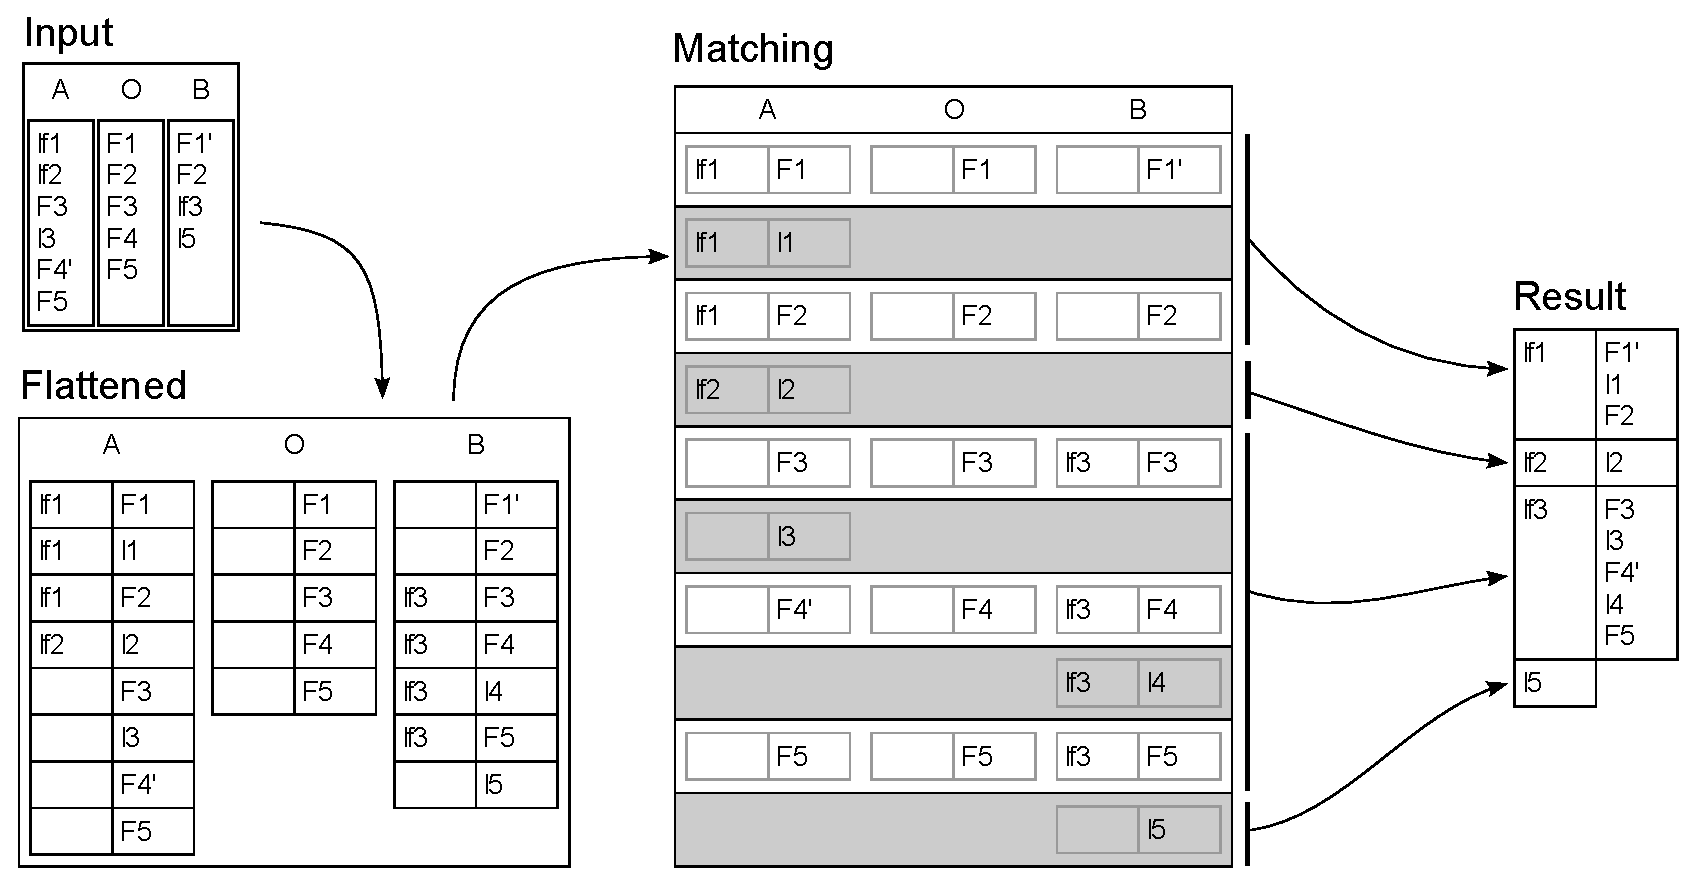
\includegraphics[scale=0.55]{drawings/html/EditedFlattenedMerge.eps}}
   \caption{Process of merging uneven trees.}
   \label{UeventreeProcess}
\end{figure}

\paragraph{Flattening} MergeUneven starts by flattening the input lists, in the sense that for any node found in the input lists that contains a substatement or a block, we bring these statements into the top level. During the flattening we remember the parent of each node, as can be seen in the left columns of the Flattened-item in the figure. Looking at the flattened list of child and parent elements,  it is obvious that chunks of continuous parent items in any of the three lists is a sub-block.

\paragraph{Matching} Afterwards we run PriorityChunking on the child elements of the flattened lists. If some statements have been moved to a subscope for these conflicts, this matches these statements with the ones in the other branches scope. As mentioned above, a continuous sequence of keys in the three branches means a sub-block. The same is the case in this matching: For each branch, we are able to track opening and closing sub-scopes by looking at the change between the last observed parent element, and at the current. This means we can isolate chunks of matches that happen in specific scopes. After isolating these, we can merge the parents, and for each continuous sequence of parent items, we can output a block around them.

\paragraph{Running time} This algorithm is dominated by PriorityChunking, which runs in $O(n^2(t+t'))$ time. In this case $t$ is equality, running $O(n)$ time and $t'$ is similarity, running $O(n^4)$ time, giving an overall running time of $O(n^3+n^6)$.

\subsubsection{Running time}
While merging a syntax tree, our worst case scenario is to visit every node in all three input trees one time. For each visit to a node, we will be doing some work, depending on what kind of node it is:

\begin{itemize}
\item If it is a fixed structural node, each node will run in $O(1)$; excluding the recursive call.
\item If it is a list-node, each node will perform an unordered matching on the input lists; taking $t_u$ time.
\item If it is a block-node, each node will perform an ordered matching on the input lists; taking $t_o$ time.
\end{itemize}

The above running times is excluding the work that the recursive calls will make; only describing what work will be contributed to the running time by each node. If $n$ is the sum of nodes in all three input trees, A, O and B, the overall running time will be:

\begin{equation}
O(n \cdot \max(t_u, t_o)) \nonumber
\end{equation}

\paragraph{MergeList} MergeList is dominated by the running time of cost-matching, which is $O(m^2 \log m)$, where $m$ is the biggest of the three input sets. $m$ is smaller than $n$ in our case; any list in the three must be smaller than the size of the tree. We get an overall time for $t_u$ to be $O(m^2 \log m)$.

\paragraph{MergeBlock} MergeBlock runs PriorityChunk, which has the running time of $O(|O| (|A| + |B|)(t + t'))$ where A, O and B is the input sequences, and $t$ and $t'$ is the running time of equality and similarity; in our case $t$ is $O(n)$ and $t'$ is $O(n^4)$. If we upper bound $|A|$, $|O|$ and $|B|$ as $n$, we get an overall running time of:

\begin{equation}
O(n (n + n)(n + n^4)) \nonumber
\end{equation}

Which can be simplified into:

\begin{equation}
O(n^3 + n^6) \nonumber
\end{equation}

Note in this expression that $n^3$ is due to the equality-stable chunk, and that $n^6$ is due to similarity-stable chunks; because of this we decide not to throw away $n^3$ because it will later allow us to argue about the overall running time of our algorithm.

\paragraph{MergeNode} The overall running time for MergeNode thus become:
\begin{equation}
O(n^4 + n^7) \nonumber
\end{equation}


\subsection{Running time}
In this section we will give a brief overview of the overall running time of the algorithm we have created. In Table \ref{RunningTimeTable}, we generally view $n$ as $O(max(|A|, |O|, |B|)$, $O(max(|X|, |Y|)$  or $O(|M|)$ depending on the input parameters. $t$ and $t'$ are the running times of input functions in order.

Further, it can be said:

\begin{enumerate}
\item For MergeFile, $c$ is the running time of its internal conflicthandler; MergeSyntax.
\item For MergeSyntax, $m$ is the number of matches. $c$ is the running time of the conflict-handler; MergeSequence and MergeNode if a conflicts happens.
\end{enumerate}

\begin{table}
\begin{tabular}{l | l  }
\textbf{Algorithm} & \textbf{Upper bound} \\ \hline
TwoWayMatching(X, Y, eq) & $O(n^2 \cdot t)$ \\
ThreeWayMatching(A, O, B, eq) & $O(n^2 \cdot t)$ \\
Chunking(M) & $O(n)$ \\
PriorityChunking(A, O, B, eq, sim) & $O(n^2(t + t')$ \\
TwoWayCostMatching(X, Y, cost) & $O(n^2 \log n)$ \\
ThreeWayCostMatching(A, O, B, cost) & $O(n^2 \log n)$ \\
Reordering(A, O, B) & $O(n^2)$ \\

MergeSequence(A, O, B, eq, ch) & $O(n^2 \cdot t)$  or  $O(n^2 \cdot t +  t')$ \\

Equality(X, Y) & $O(n)$ \\
Similar(X, Y) & $O(n^4)$ \\


MergeFile(A, O, B) & $O(n^2 + c)$ \\
MergeSyntax(A, O, B) & $O(n^3 \log n + m \cdot c)$ \\
MergeNode(A, O, B) & $O(n^4 + n^7)$ \\
MergeUneven(A, O, B) & $O(n^3 + n^6)$ \\
\end{tabular}
\caption{Running times for all algorithms}
\label{RunningTimeTable}
\end{table}

In the below we use three variables to define the input sizes. $l$ is number of lines of a file, $n_s$ is the number of nodes used to structure a code file, $l_f$ is the number of lines in a function and $n_f$ is the number of nodes in a function. $m$ is the number of matches from the structure matcher. The overall upper bound for our entire algorithm becomes:

\begin{equation}
O(l^2 + n_s^3 \log n_s + m ( l_{f}^2 + n_{f}^4 + n_{f}^7)) \nonumber
\end{equation}

A couple of notes about this running time:

\begin{itemize}
	\item Most of the running time are quite crude upper bounds.
	\item For most files in a commit, more often than not the running time will be $l^2$, due to the sequence-merging succeeding.
	\item For most matches, the running time is $l_f^2$ due to sequence-merging succeeding on this function.
	\item In the running from MergeNode, $O(n^4 + n^7)$, the $n^7$ part only happens when there is no equality in the tree; which hopefully happens only a few times in the entire merge.
\end{itemize}

\begin{comment}

\subsection{Merging examples}
Here we will provide some examples of runs of the implemented merging algorithm for some source written in C\#. 

\begin{sidewaysfigure}
Reordering parameters and arguments in one branch, while inserting a new in another:
\begin{multicols*}{4}
\textbf{A}
\begin{lstlisting}[language=CSharp]
void F(string b, int a)
{
F('test', 1);
}
\end{lstlisting}
\columnbreak

\textbf{O}
\begin{lstlisting}[language=CSharp]
void F(int a, string b)
{
F(1, 'test');
}   
\end{lstlisting}
\columnbreak

\textbf{B}
\begin{lstlisting}[language=CSharp]
F(int a, string b, int i)
{
F(1, 'test', 2);
}
\end{lstlisting}
\columnbreak

\textbf{Result}
\begin{lstlisting}[language=CSharp]
F(int a, string b, int i)
{
F(1, 'test', 2);
}
\end{lstlisting}
\end{multicols*}


Method call changed in one branch, and parameter changed in the other branch.
\begin{multicols*}{4}
\textbf{A}
\begin{lstlisting}[language=CSharp]
void F()
{
	O.G(""N"");
}
\end{lstlisting}
\columnbreak

\textbf{O}
\begin{lstlisting}[language=CSharp]
void F()
{
	O.G(""O"");
}
\end{lstlisting}
\columnbreak

\textbf{B}
\begin{lstlisting}[language=CSharp]
void F()
{
	O.H(""O"");
}
\end{lstlisting}
\columnbreak

\textbf{Result}
\begin{lstlisting}[language=CSharp]
F(int a, string b, int i)
{
	O.H("N");
}
\end{lstlisting}
\end{multicols*}
\end{sidewaysfigure}
\end{comment}

\clearpage
\section{Future work}
Several questions are left unanswered at the end of this thesis. In this section we will give a brief overview of these.

\paragraph{Evaluation of the output merges} While we abstractly have reasoned about every single part of the solution made, we have only tried to run the algorithm on small toy examples; not on real-life scenarios. A reasonable extension of this project would be to find repositories of C\# code and evaluate how well conflicts are actually handled: if we avoid conflicts in this approach, and how well the merges we produce line up with the code that manual merging has produced in these repositories.

\paragraph{Evaluation of the actual running time} We have provided an analysis that shows the asymptotic upper bound for an entire run of the algorithm in big O notation, and have provided arguments for why the most time consuming parts of the algorithm is only rarely hit. This is reasonable first step, however big O is also a quite forgiving measurement and this analysis by no means provides evidence that the algorithm will perform well in real-life scenarios. Evaluating the actual running time of the algorithm on real-life source code, as well as source code constructed to trigger the most time consuming parts of the algorithm.

\paragraph{Better structure matching and merging} The structure matcher that we provide is quite limited; most notably it cannot match members of classes or namespaces if they have been moved to another parent node. Further it only considers the identifiers for the namespaces or classs that are being compared; this give a quite big potential for problems when restructuring the namespace- and class-hierarchies in files.

Line based merging has fewer difficulties in this regard; when restructuring happens in one branch, this branch will only be changing the lines that make up the structure; the rest of the lines are unaffected, and if another branch has made changes within functions, this will be merged perfectly.

\paragraph{Renaming} As noted in Section \ref{TrivialConflict} one scenario of trivial conflicts that we could have looked into could be what happens with variable renaming. 

\paragraph{Whitespace, comments and preprocessing directives} As noted in Section \ref{PreprocessComments} the syntax tree abstracts detail like comments, whitespace and preprocessing directives out. This will not be a problem for the line based merging that we do, however we have not considered this in our structural merge; our returned code will be completely stripped of comments, preprocessing and whitespace. Enabling this would however be essential for this to be practically useful.

\paragraph{Stable reordering} As noted in Section \ref{ThreeWayReorderingAlgorithmSec} the behaviour of our reordering function depends heavily on the result of three-way sequence matching, which unfortunately is a little ambiguous due to our two-way sequence matching algorithm only providing one of the possible results of the input sequences instead of all of them.

\paragraph{Cost-based two-way sequence matching} The abstraction we made over Needlemann-Wunch allowing only a specific cost-scheme based on a boolean function has simplified our matchings considerably. However, Needlemann-Wunch also provide the ability to define costs between items in the input sequences. This might be useful, and lower the running time of our algorithm, if used in the priority-chunking function.

\clearpage
\section{Conclusion}
In this thesis we have investigated the topic of automatic merging of source code using structure awareness to resolve conflicts.

We found that automatic conflict-resolution cannot be a goal in itself with a structure aware tool, and defined four specific scenarios where a structure aware tool could be more forgiving with merging than a line-based tool: Reordered class members, reordering parameter lists and argument lists, merging statements where different lines have changed and merging when an identifier has changed. Of these four scenarios, we implemented three of these four scenarios.

We found that generally tree-merging of complete syntax trees is not practical in version control due to time consumption being much higher for tree merging than sequence merging. As a consequence we created an algorithm that relied on tree merging only as a last resort, after trying line-based merging on both entire files and individual methods.

We divided the process of merging syntax trees into two processes: class-merging and method-merging. The merging classes is done by unordered matching of methods; thereby resolving conflicts caused by moving methods around within classes. When doing structured merging of method, we created an algorithm that would investigate match not only if nodes are equal, but also if they are similar enough to be merged; thereby we created an algorithm that allowed us to merge on a much more fine grained level than lines.

While we have substantiated our decisions and analysed the consequences of our choices throughout the thesis, we have yet to run tests of real life code on the algorithm, as such we cannot provide any empirical evidence to how well this algorithm actually performs.

\clearpage

\listofalgorithms

\clearpage

\bibliographystyle{plainnat}
\bibliography{libary}

\end{document}

